% Compile with XeLaTeX or LuaLaTeX
\documentclass[10pt]{article}  % Spivak uses ~10pt

% -----------------------------
% Fonts
% -----------------------------
\usepackage{fontspec}
\setmainfont{TeX Gyre Pagella}
\usepackage{unicode-math}
\setmathfont{Libertinus Math}

% -----------------------------
% Page layout
% -----------------------------
\usepackage[margin=2.5cm]{geometry}
\usepackage[parfill]{parskip}

% -----------------------------
% Theorems and QED
% -----------------------------
\usepackage{amsthm}
\usepackage{tcolorbox}
\tcbuselibrary{breakable}

% QED symbol like Spivak (tall gray rectangle)
\renewcommand{\qedsymbol}{\textcolor{black}{\rule{1ex}{2.2ex}}}

\newtheorem{theorem}{Theorem}
\newtheorem{axiom}{Axiom}
\newtheorem{definition}{Definition}

% -----------------------------
% Misc packages
% -----------------------------
\usepackage{graphicx, subfig}
\usepackage{booktabs, array}
\usepackage{paralist, verbatim}
\usepackage{xcolor, pagecolor}
\usepackage{fancyhdr}
\pagestyle{fancy}
\renewcommand{\headrulewidth}{0pt}
\lhead{}\chead{}\rhead{}
\lfoot{}\cfoot{\thepage}\rfoot{}
\usepackage{sectsty}
\allsectionsfont{\sffamily\mdseries\upshape}
\usepackage[nottoc,notlof,notlot]{tocbibind}
\usepackage[titles,subfigure]{tocloft}
\renewcommand{\cftsecfont}{\rmfamily\mdseries\upshape}
\renewcommand{\cftsecpagefont}{\rmfamily\mdseries\upshape}
\usepackage{changepage, comment}
% Define a light gray
\definecolor{lightgraypaper}{RGB}{240,240,240}
% Set the page background
\pagecolor{lightgraypaper}
\color{black} % keep text black

\title{Title by Author}
\author{Noah Lewis}
\begin{document}
\maketitle

\tableofcontents

\section{The Natural Numbers}
\begin{tcolorbox}[title=Problem 1, breakable]
    Prove using mathematical induction that for all positive integers $n$,
    \[1 + 2 + 3 + \cdots + n = \frac{n(n + 1)}{2}\]
\end{tcolorbox}

\begin{proof}
    Let $n = 1$ then $\frac{n(n + 1)}{2} = \frac{1(1 + 1)}{2} = \frac{1(2)}{2} = 1$.
    Assume the formula is true for some integer $k = n - 1$, thus:
    \begin{align*}
        1 + 2 + 3 + \cdots + (n - 1) = \frac{(n - 1)((n - 1) + 1)}{2}
    \end{align*}
    Thus:
    \begin{align*}
         & 1 + 2 + 3 + \cdots + (n - 1) + n               \\
         & = \frac{(n - 1)((n - 1) + 1)}{2} + n           \\
         & = \frac{{(n - 1)}^2 + n - 1}{2} + \frac{2n}{2} \\
         & = \frac{{(n - 1)}^2 + 3n - 1}{2}               \\
         & = \frac{n^2 - 2n + 1 + 3n - 1}{2}              \\
         & = \frac{n(n + 1)}{2}
    \end{align*}
\end{proof}

\begin{tcolorbox}[title=Problem 3, breakable]
    You probably recall from your previous mathematical work the \emph{triangle inequality:}
    for any real numbers $x$ and $y$,
    \[|x + y| \le |x| + |y|\]
    Accepts this as given (or see a calculus text to recall how it is proved).
    Generalize the triangle inequality, by proving that 
    \[|x_1 + x_2 + \cdots + x_n \le |x_1| + |x_2| + \cdots |x_n|,\]
    for any positive integer $n$.
\end{tcolorbox}

\begin{proof}
    For $n = 1$, trivially $|x_1| \le |x_1|$.
    For $n = 2$, $|x_1 + x_2| \le |x_1| + |x_2|$ by the triangle inequality.
    Now assume the formula holds for $k = n - 1$, thus:
    \begin{align*}
        |x_1 + x_2 + \cdots + x_{n - 1}| \le |x_1| + |x_2| + \cdots |x_{n - 1}|
    \end{align*}
    Thus:
    \begin{align*}
         & |x_1 + x_2 + \cdots + x_{n - 1} + x_n|        &  &                                  \\
         & \le  |(x_1 + x_2 + \cdots + x_{n - 1}) + x_n| &  &                                  \\
         & \le  |x_1 + x_2 + \cdots + x_{n - 1}| + |x_n| &  & \quad \text{triangle inequality} \\
         & \le  |x_1| + |x_2| + \cdots + |x_n|           &  & 
    \end{align*}
\end{proof}

\begin{tcolorbox}[title=Problem 4, breakable]
    Given a positive integer $n$, recall that $n! = 1 \cdot 2 \cdot 3 \cdots$ (this is read as 
    $n$ factorial). Provide an inductive definition for $n!$. (It  is customary to actually 
    start this defintion at $n = 0$, setting $0! = 1$) 
\end{tcolorbox}

\textbf{Solution}

We can define $n!$ as follows. If $n <=1$, then $n! = 1$. If $n > 1$, then $n!
    = n(n - 1)!$.

\begin{tcolorbox}[title=Problem 5, breakable]
    Prove that $2^n < n!$ for all $n \ge 4$.
\end{tcolorbox}

\begin{proof}
    Let $n = 4$, then $2^4 = 16 < 4! = 24$.
    Assume the inequality holds for $k = n - 1$, thus:
    \begin{align*}
        2^{n - 1} < (n - 1)!
    \end{align*}
    Thus:
    \begin{align*}
         & 2^{n - 1} \cdot 2 < (n - 1)! \cdot n \quad \text{Note: $2 < 4 \le n$} \\
         & 2^n < n! 
    \end{align*}
\end{proof}

\begin{tcolorbox}[title=Problem 7, breakable]
    Prove the familiar geometric progression formula.
    Namely, suppose that $a$ and $r$ are real numbers with $r \not = 1$.
    Then show that:
    \[a + ar  + ar^2 + \cdots + ar^{n - 1} = \frac{a - ar^n}{1 - r}\]
\end{tcolorbox}

\begin{proof}
    Let $n = 1$, then $a = \frac{a - ar^n}{1 - r} = \frac{a - ar}{1 - r} = \frac{a(1 - r)}{1 - r} = a$.
    Assume the formula holds for $k = n - 1$, thus:
    \[a + ar + ar^2 + \cdots + ar^{n - 2} = \frac{a - ar^{n - 1}}{1 - r}\]
    Thus
    \begin{align*}
         & a + ar + ar^2 + \cdots + ar^{n - 2} + ar^{n - 1}                \\
         & =\frac{a - ar^{n - 1}}{1 - r} + ar^{n - 1}                      \\
         & =\frac{a - ar^{n - 1}}{1 - r} + \frac{(1 - r)ar^{n - 1}}{1 - r} \\
         & =\frac{a - ar^{n - 1} + (1 - r)(ar^{n - 1})}{1 - r}             \\
         & =\frac{a - ar^{n - 1} + ar^{n - 1} - ar^n}{1 - r}               \\
         & =\frac{a - ar^n}{1 - r}
    \end{align*}
\end{proof}

\begin{tcolorbox}[title=Problem 12, breakable]
    Consider the sequence ${a_n}$ defined inductively as follows:
    \[a_1 = 5, a_2  = 7, a_{n + 2} = 3a_{n + 1} - 2a_n\]
\end{tcolorbox}

\begin{proof}
    Let $n = 1$, then $a_1 = 5 = 3 + 2^n =  3 + 2^1 = 5$.
    Let $n = 2$, then $a_2 = 7 = 3 + 2^n = 3 + 2^2 = 7$
    Assume the formula holds for $k < n$ thus:
    \[a_{n - 1} = 3 + 2^{n - 1}\]
    and 
    \[a_{n - 2} = 3 + 2^{n - 2}\]
    So $k = n$ is:
    \[a_{n} = 3a_{n - 1} - 2a_{n - 2} = 3(3 + 2^{n - 1}) - 2(3 + 2^{n - 2})\]
    Then:
    \begin{align*}
         & 3(3 + 2^{n - 1}) - 2(3 + 2^{n - 2})             \\
         & = 9 + 3 \cdot 2^{n - 1} - 6 - 2 \cdot 2^{n - 2} \\
         & = 3 + 3 \cdot 2^{n - 1} - 2^{n - 1}             \\
         & = 3 + 2 \cdot 2^{n - 1}                         \\
         & = 3 + 2^n                            
    \end{align*}
\end{proof}

\begin{tcolorbox}[title=Problem 14, breakable]
    In this problem you will prove some results about the binomial coefficients, using induction.
    Recall that:
    \[\binom{n}{k} = \frac{n!}{(n - k)!k!}\]
    where $n$ is a positive integer, and $0 \le k \le n$.

    (a) Prove that 
    \[\binom{n}{k} = \binom{n - 1}{k} + \binom{n - 1}{k - 1}\]
    $n \ge 2$ and $k < n$. Hint: You do not need induction to prove this.
    Bear in mind that $0! = 1$.

    (b) Verify that $\binom{n}{0} = 1$ and $\binom{n}{n} = 1$. Use these facts,
    together with part a, to prove by induction on $n$ that $\binom{n}{k}$ is an integer,
    for all $k$ with $0 \le k \le n$. (Note: You may have encountered $\binom{n}{k}$ as the 
    count of the number of $k$ element subsets of a set of $n$ objects; it follows that from this 
    $\binom{n}{k}$ is an integer. What we are asking for here is an inductive proof based on algebra.)

    (c) Use part a and induction to prove the Binomical Theorem: For non-negative $n$ and variables $x$, $y$,
    \[{(x + y)}^n = \sum_{k = 0}^{n} \binom{n}{k}x^{n - k}y^k\]
\end{tcolorbox}

\begin{proof}
    \begin{align*}
         & \binom{n - 1}{k} + \binom{n - 1}{k - 1}                                                             \\
         & = \frac{(n - 1)!}{((n - 1) - k)!k!} + \frac{(n - 1)!}{((n - 1) - (k - 1))!(k - 1)!}                 \\
         & =  (n - 1)!\left(\frac{1}{((n - 1) - k)!k!} + \frac{1}{((n - 1) - (k - 1))!(k - 1)!}\right)         \\
         & =  (n - 1)!\left(\frac{1}{((n - 1) - k)!k(k - 1)!} + \frac{1}{((n - 1) - (k - 1))!(k - 1)!}\right)  \\
         & =  \frac{(n - 1)!}{(k - 1)!}\left(\frac{1}{((n - 1) - k)!k} + \frac{1}{((n - 1) - (k - 1))!}\right) \\
         & =  \frac{(n - 1)!}{(k - 1)!}\left(\frac{1}{(n - k - 1)!k} + \frac{1}{(n - k)!}\right)               \\
         & =  \frac{(n - 1)!}{(k - 1)!}\left(\frac{1}{(n - k - 1)!k} + \frac{1}{(n - k)(n - k - 1)!}\right)    \\
         & =  \frac{(n - 1)!}{(k - 1)!(n - k - 1)!}\left(\frac{1}{k} + \frac{1}{(n - k)}\right)                \\
         & =  \frac{(n - 1)!}{(k - 1)!(n - k - 1)!}\left(\frac{n - k}{k(n - k)} + \frac{k}{k(n - k)}\right)    \\
         & =  \frac{(n - 1)!}{(k - 1)!(n - k - 1)!}\left(\frac{n}{k(n - k)}\right)                             \\
         & =  \frac{n!}{k!(n - k)!}
    \end{align*}
\end{proof}

\begin{proof}
    Let $k = 0$ then, $\binom{n}{0} = \frac{n!}{(n - 0)!(0!)} = \frac{n!}{n!} = 1 \in \mathbb{Z}$.
    Let $k = n$ then, $\binom{n}{n} = \frac{n!}{(n - n)!(n!)} = \frac{n!}{n!} = 1 \in \mathbb{Z}$.
    Assume this holds for $n - 1$, thus for all $k$ where $0 \le k \le n - 1$:
    \[\binom{n - 1}{k} \in \mathbb{Z}\]
    Then:
    \[\binom{n}{k} =  \binom{n - 1}{k} + \binom{n - 1}{k - 1}\]
    Since each of these terms exist in $\mathbb{Z}$ their sum $\binom{n}{k}$ is in
    $\mathbb{Z}$ since the integers are closed over addition.
\end{proof}

\begin{proof}
    Let $n = 0$. Then:
    \begin{align*}
        {(x + y)}^0 = 1 = \sum_{k = 0}^{0} \binom{0}{k} x^k y^{0-k} = \binom{0}{0} x^0 y^0 = 1 \cdot 1 \cdot 1 = 1
    \end{align*}

    Assume the formula holds for $n - 1$, thus:
    \begin{align*}
        \sum_{k = 0}^{n - 1} \binom{n - 1}{k} x^k y^{(n-1)-k} = (x+y)^{n - 1}
    \end{align*}
    Then:
    \begin{align*}
        {(x+y)}^n & = {(x+y)}^{n - 1} \cdot (x + y)  s                                                                                              \\
                  & = \left(\sum_{k = 0}^{n - 1} \binom{n - 1}{k} x^k y^{(n-1)-k}\right) \cdot (x + y)                                              \\
                  & = x \cdot \sum_{k = 0}^{n - 1} \binom{n - 1}{k} x^k y^{(n-1)-k} + y \cdot \sum_{k = 0}^{n - 1} \binom{n - 1}{k} x^k y^{(n-1)-k} \\
                  & = \sum_{k = 1}^{n} \binom{n - 1}{k - 1} x^k y^{n - k} + \sum_{k = 0}^{n - 1} \binom{n - 1}{k} x^k y^{n - k}                     \\
                  & = \sum_{k = 0}^{n} \left( \binom{n - 1}{k - 1} + \binom{n - 1}{k} \right) x^k y^{n - k}                                         \\
                  & = \sum_{k = 0}^{n} \binom{n}{k} x^k y^{n - k}
    \end{align*}
\end{proof}

\begin{tcolorbox}[title=Problem 15, breakable]
    Criticize the following ``proof'' showing that all cows are the same
    color.

    It suffices to show that any herd of $n$ cows has the same color. If the herd
    has but one cow, then trivially all the cows in the herd have the same color.
    Now suppose that we have a herd of n cows and $n > 1$. Pick out a cow and
    remove it from the herd, leaving $n - 1$ cows; by the induction hypothesis
    these cows all have the same color. Now put the cow back and remove another
    cow. (We can do so because $n > 1$.) The remaining $n - 1$ again must all be
    the same color. Hence, the first cow selected and the second cow selected have
    the same color as those not selected, and so the entire herd of n cows has the
    same color.
\end{tcolorbox}

\textbf{Solution}

The proof selects a different set of $n - 1$ cows each time.

\begin{tcolorbox}[title=Problem 16, breakable]
    Prove the converse of Theorem 1.1; that is, prove that the Principle 
    of Mathematical Induction implies the Well-ordering Princple. 
    (This shows that these two principles are logically equivalent,
    and so from an axiomatic point of view it doesn't matter which
    we assume is an axiom for the natural numbers.)
\end{tcolorbox}

\begin{proof}
    Assume that the principle of mathematical induction holds.
    Let $G \subseteq \mathbb{N}$ be nonempty. For contradiction, suppose $G$ has no least element. 
    Define $P(n)$ to be the statement: ``Nothing $\le n$ is in $G$.''

    If $1 \in G$, then $1$ would be the least element of $G$, a contradiction. So
    $1 \notin G$ and $P(1)$ is true.

    Assume $P(n)$ holds meaning no element of $G$ is $\le n$. If $n+1 \in G$, then
    $n+1$ would be the least element of $G$, a contradiction. Therefore $n+1 \notin
        G$, and hence $P(n+1)$ holds.

    By induction, $P(n)$ holds for all $n \in \mathbb{N}$. So no element of
    $\mathbb{N}$ is in $G$, so $G = \emptyset$, contradicting the assumption that
    $G$ is nonempty. 
\end{proof}
\section{The Integers}
\begin{tcolorbox}[title=Problem 3, breakable]
    Prove that the set of all linear combinations of $a$ and $b$
    are precisely the multiple of $\gcd(a, b)$.
\end{tcolorbox}

\begin{proof}
    Let $a, b$ be integers such that $a \not = 0$ or $b \not = 0$.
    We know $ax + by = \gcd(a, b)$ for some $x, y \in \mathbb{Z}$.
    Let $t$ be an arbitrary integer.
    Then $t(ax + by) = t(\gcd(a, b))$.
    It follows that $a(tx) + b(ty) = t(\gcd(a, b))$
    Showing that any integer multiple $t$ of the $\gcd(a, b)$
    is equivalent to some linear combination of $a, b$.

    Let $a$, $b$, $x$, and $y$ be arbitrary integers.
    Let $d = \gcd(a, b)$. It follows that $d \mid a$ and $d \mid b$.
    Then $a = dt$ for some $t \in \mathbb{Z}$ and $b = df$ for some $f \in \mathbb{Z}$.
    Then:
    \begin{align*}
        ax + by = dtx  + dfy = d(tx + fy)
    \end{align*}
    So any linear combination of $a$ and $b$ is a multiple of the $\gcd(a, b)$.
\end{proof}

\begin{tcolorbox}[title=Problem 4, breakable]
    Two numbers are said to be relatively prime if their $\gcd$ is $1$.
    Prove $a, b$ relatively prime if and only if every integer can be written
    as a linear combination of $a$ and $b$.
\end{tcolorbox}

\begin{proof}
    $\rightarrow$ Suppose $a, b \in \mathbb{Z}$ are relatively prime.
    Let $d \in \mathbb{Z}$. Since $a, b$ are relatively prime $\gcd(a, b) = ax + by = 1$ where $x, y \in \mathbb{Z}$.
    Then $d(\gcd(a, b)) = d(ax + by) = a(dx) + b(dy) = d(1) = d$.

    $\leftarrow$ Suppose every integer can be written as a linear combination of $a$ and $b$.
    In particular $1 = ax + by$ for some $x, y \in \mathbb{Z}$.
    Then $\gcd(a, b) = 1 = ax + by$ so $a$ and $b$ are relatively prime.
\end{proof}

\begin{tcolorbox}[title=Problem 5, breakable]
    Prove Theorem $2.6$. That is, use induction to prove that if the 
    prime $p$ divides $a_1 a_2 \cdots a_n$, then $p$ divides $a_i$ for some $i$.
\end{tcolorbox}

\begin{proof}
    Suppose $p$ is prime.

    Base case: If $p \mid a_1 a_2$ by definition of being prime $p \mid a_1$ or $p \mid a_2$.

    Assume the Theorem holds for $n - 1$ so if $p \mid a_1 a_2 \cdots a_{n - 1}$ then $p \mid a_i$
    for some $i$. Now suppose $p \mid a_1 a_2 \cdots a_{n - 1} a_n$. Let $c = a_1 a_2 \cdots a_{n - 1}$,
    then $p \mid c \cdot a_n$. By definition of being prime $p \mid c$ by the induction hypothesis or $p \mid a_n$.
\end{proof}

\begin{tcolorbox}[title=Problem 6, breakable]
    Suppose that $a$ and $b$ are positive integers.
    If $a + b$ is prime, prove that $\gcd(a, b) = 1$.
\end{tcolorbox}

\begin{proof}
    We've already proved $n$ is prime iff $n$ is irreducible.
    Suppose $a + b$ is prime and for contradiction $\gcd(a, b) = x > 1$.
    Since $a + b$ is prime it has no factors other than itself and $1$.
    Since $\gcd(a, b) = x > 1$ then $x \mid a $ and $x \mid b$.
    Furthermore, $a = tx$ and $b = yx$ for some $t, y \in \mathbb{Z}$.
    Then $a + b = tx + yx = x(t + y)$ a contradiction since $a + b$ is prime.
\end{proof}

\begin{tcolorbox}[title=Problem 7, breakable]
    (a) A natural number greater than $1$ that is not prime 
    is called composite. Show that for any $n$, there is a run 
    of $n$ consecutive composite numbers. Hint: Think Factorial.
    
    (b) Therefore, there is a string of $5$ consecutive composite numbers 
        starting where?
\end{tcolorbox}

\begin{proof}
    Let $T = \{2, 3, \ldots, n + 1\}$ and let $i$ be an element in $T$.
    Now let 
    \[
        d = i + (n+1)!.
    \]
    First notice $2 \le i \le n + 1$. Then:
    \begin{align*}
        ((i + 1) + (n+1)!) - (i + (n+1)!) = 1
    \end{align*}
    Showing consecutive values of $i$ produce consecutive values of $d$. 
    Since $2 \le i \le n+1$, we have $i \mid (n+1)!$.
    Then:
    \begin{align*}
        d &= i + (n+1)! \\
          &= i \left( 1 + \frac{(n+1)!}{i} \right)
    \end{align*}
    Clearly $d$ is a composite number since it has been factored into $2$ integers greater than 1.
    Thus, the $n$ values of $d$ produce a sequence of $n$ consecutive composite numbers.
\end{proof}

\textbf{Solution (b):}

\[722 = 2 \cdot 361, 723 = 3 \cdot 241, 724 = 2 \cdot 362, 725 = 5 \cdot 145, 726 = 2 \cdot 363\]

\begin{tcolorbox}[title=Problem 9, breakable]
    Notice that $\gcd(30, 50) = 5\gcd(6, 10) = 5 \cdot 2$. In fact, this is 
    always true; prove that if $a > 0$, then $\gcd(ab, ac) = a \cdot \gcd(b, c)$.
\end{tcolorbox}

\begin{proof}
    Let $p = \gcd(ab, ac) = abx + acy$. Since $a \mid p$ there exists $r$ such that $p = ar$.
    So $ar = abx + acy$ and dividing by $a$ gives $r = bx + cy$. 
    Since $a > 0$
        and $ar = \gcd (ab,ac) > 0$ it follows that $r > 0$. 
    Thus $r$ is a positive linear combination of $b$ and $c$.
    Suppose, for contradiction, there exists $d$ that is a positive linear combination of $b$ and $c$, and $d < r$.
    So $d = bu + cv$ for some integers $u, v$.
    Since $a > 0$ it follows that $ad > 0$.
    But then $ad = abu + acv$ and $ad < ar = p$ contrdicting the minimality of $p$.
    Therefore $r = \gcd(b, c)$.
    It follows that $\gcd(ab, ac) = ar =  a \cdot \gcd(b, c)$.
\end{proof}

\begin{tcolorbox}[title=Problem 10, breakable]
    Suppose two integers $a$ and $b$ have been factored into primes as follows:
    \[a = p_1^{n_1} p_2^{n_2} \cdots p_r^{n_r}\]
    and 
     \[b = p_1^{m_1} p_2^{m_2} \cdots p_r^{m_r}\]
    where the $p_i$'s are primes, and the exponents $m_i$ and $n_i$ are non-negative 
    integers. It is the case that 
    \[\gcd(a, b) = p_1^{s_1} p_2^{s_2} \cdots p_r^{s_r}\]
    where $s_i$ is the smaller of $n_i$ and $m_i$. Show this with $a = 360 = 2^3 \cdot 3^2 \cdot 5$
    and $b = 2^2 3^2 5^2$. Now prove this fact in general.
\end{tcolorbox}

\textbf{Solution:}

Let 
\[
a = 360 = 2^3 \cdot 3^2 \cdot 5^1, \quad
b = 2^2 \cdot 3^2 \cdot 5^2.
\]
\textbf{Exponents of each prime factor:}
\[
\begin{array}{c|c|c}
\text{Prime } p_i & \text{Exponent in } a \ (n_i) & \text{Exponent in } b \ (m_i) \\
\hline
2 & 3 & 2 \\
3 & 2 & 2 \\
5 & 1 & 2
\end{array}
\]
\textbf{Minimum exponent for each prime:}
\[
s_i = \min(n_i, m_i)
\]
\[
\begin{array}{c|c}
\text{Prime } p_i & s_i = \min(n_i, m_i) \\
\hline
2 & 2 \\
3 & 2 \\
5 & 1
\end{array}
\]
\textbf{Multiply the primes raised to the minimum exponents:}
\[
\gcd(a,b) = 2^2 \cdot 3^2 \cdot 5^1 = 4 \cdot 9 \cdot 5 = 180.
\]
The gcd of $360$ and $900$ is $180$.

\begin{proof}
    Let $a = \prod_{i=1}^r p_i^{n_i}$ and $b = \prod_{i=1}^r p_i^{m_i}$.
    For each prime $p_i$, define $s_i = \min(n_i, m_i)$ and let $c_i = p_i^{s_i}$. 

    First note that the $\gcd$ will have the common prime factors of $a$ and $b$.
    A prime not common to both would not divide both.

    Let $f_i = p_i^{s_i + 1}$ for the $i$th prime number appearing in $a$ and $b$. 
    Then $f_i > p_i^{m_i}$ or $f_i > p_i^{n_i}$ so $f_i \nmid p_i^{m_i}$ or $f_i \nmid p_i^{n_i}$.
    So $c_i$ is the largest power of $p_i$ dividing the $i$th prime of both numbers.

    Since the primes are independent, the greatest common divisor of $a$ and $b$ is 
        $\gcd(a,b) = \prod_{i=1}^r c_i = \prod_{i=1}^r p_i^{s_i}$.
\end{proof}

\begin{tcolorbox}[title=Problem 11, breakable]
    The \textbf{least common multiple} of natural numbers $a$ and $b$
    is the smallest positive common multiple of $a$ and $b$. That is,
    if $m$ is the least common mulitple of $a$ and $b$, then $a \mid m$
    and $b \mid m$, and if $a \mid n$ and $b \mid n$ then $n \ge m$.
    We will write $lcm(a, b)$ for the least common mulitple of $a$ and $b$.
    Can you find a formula for the lcm of the type given for the gcd in 
    the previous excersize.
\end{tcolorbox}

\textbf{Solution}

Suppose two integers $a$ and $b$ have been factored into primes as follows:
\[a = p_1^{n_1} p_2^{n_2} \cdots p_r^{n_r}\]
and 
\[b = p_1^{m_1} p_2^{m_2} \cdots p_r^{m_r}\]
where the $p_i$'s are primes, and the exponents $m_i$ and $n_i$ are non-negative 
integers. It is the case that 
\[lcm(a, b) = p_1^{s_1} p_2^{s_2} \cdots p_r^{s_r}\]
where $s_i$ is the larger of $n_i$ and $m_i$.

\begin{tcolorbox}[title=Problem 12, breakable]
    Show that if $\gcd(a, b) = 1$, then $lcm(a, b) = ab$.

    In general, show that:
    \[lcm(a, b) = \frac{ab}{\gcd(a, b)}\]
\end{tcolorbox}

\begin{proof}
    We prove the general case first.

    Let $a = \prod_{i=1}^r p_i^{n_i}$ and $b = \prod_{i=1}^r p_i^{m_i}$.
    So 
    \[
        ab = \prod_{i=1}^r p_i^{n_i+m_i}.
    \]
    Now inspecting the $i$th prime in $ab$ we get $p_i^{n_i + m_i}$.
    Then looking at the $\operatorname{\gcd}$'s $i$th prime we get $p_i^{\min\{n_i, m_i\}}$.
    Suppose wlog that $n_i \geq m_i$.
    Then 
    \[
        \frac{p_i^{n_i + m_i}}{p_i^{\min\{n_i, m_i\}}} 
        = \frac{p_i^{n_i + m_i}}{p_i^{m_i}}
        = p_i^{n_i + m_i - m_i}
        = p_i^{n_i}
        = p_i^{\max\{n_i, m_i\}}.
    \]
    This is the $i$th prime factor of the $lcm$.
\end{proof}

\begin{proof}
    Suppose that for each prime $p_i$, $p_i$ divides $a$ or $b$ but not both.  
    Then for the $i$th prime factor $p_i$, either $n_i = 0$ or $m_i = 0$. 
    Then:
    \[
        \frac{p_i^{n_i + m_i}}{p_i^{\min\{n_i, m_i\}}} 
        = \frac{p_i^{n_i + m_i}}{p_i^0}
        = p_i^{n_i + m_i - 0}
        = p_i^{n_i + m_i}
        = p_i^{\max\{n_i, m_i\}}.
    \]
\end{proof}

\begin{tcolorbox}[title=Problem 13, breakable]
    Prove that if $m$ is a common multiple of both $a$ and $b$, then 
    $lcm(a, b) \mid m$.
\end{tcolorbox}

\begin{proof}
Suppose $m$ is a common multiple of both $a$ and $b$.
Then there exist integers $l$ and $f$ such that $m = la$ and $m = fb$.
Let the $i$th prime factor of $a, b, l, f$ be 
    $p_i^{n_i}$, $p_i^{m_i}$, $p_i^{t_i}$, $p_i^{s_i}$ respectively.
Then the $i$th prime factor of $m$ is
\[
m = la = p_i^{n_i+t_i}, \quad
m = fb = p_i^{m_i+s_i}.
\]
Let the $i$th prime factor of $\mathrm{lcm}(a,b)$ be $p_i^{\max\{n_i,m_i\}}$.
Then, in either case, we have
\[
n_i+t_i = m_i+s_i \ge \max\{n_i,m_i\}.
\]
So each $p_i^{\max\{n_i,m_i\}}$ divides the corresponding prime factor of $m$.
\end{proof}

\begin{tcolorbox}[title=Problem 18, breakable]
    (a) Show that in Euclid's Algorithm, the remainders are at least halved
    after two steps. That is $r_{i + 2} < 1/2 r_i$. \\

    (b) Use part a to find the maximum number of steps required for Euclid's
    algorithm. (Figure this in terms of the maximum of $a$ and $b$).
\end{tcolorbox}

\begin{proof}
    Theorem $2.3$ shows that the remainders form a strictly decreasing sequence of integers.
    Three steps of the algorithm are shown below.
    \begin{align*}
        \text{step $1$: }b_{n - 2} &= a_{n - 2} \cdot q_{n - 2} + r_{n - 2} \\
        \text{step $2$: }b_{n - 1} &= a_{n - 1} \cdot q_{n - 1} + r_{n - 1} \\
        \text{step $3$: }b_{n} &= a_{n} \cdot q_{n} + r_{n}
    \end{align*}
    Now for the $i$th iteration $b_i = a_{i - 1}$ and $a_i = r_{i - 1}$. Then:
    \begin{align*}
        \text{step $1$: }b_{n - 2} &= a_{n - 2} \cdot q_{n - 2} + r_{n - 2} \\
        \text{step $2$: }a_{n - 2} &= r_{n - 2} \cdot q_{n - 1} + r_{n - 1} \\
        \text{step $3$: }r_{n - 2} &= r_{n - 1} \cdot q_{n} + r_{n}
    \end{align*}
    Notice, in step $3$, a larger $q_n$ implies a smaller $r_n$.
    So in the worst case $q_n = 1$. So $r_{n - 2} = r_{n - 1} + r_{n} \iff r_n = r_{n - 2} - r_{n - 1}$.
    Now since $r_n < r_{n - 1}$ then $r_{n - 2} - r_{n - 1} < r_{n - 1} \iff r_{n - 2} < 2r_{n - 1}$.
    So $\frac{1}{2} r_{n - 2} < r_{n - 1}$. 
    Now since $r_n < r_{n - 2} - r_{n - 1}$ then $r_n < r_{n - 2} - \frac{1}{2} r_{n - 2} = \frac{1}{2} r_{n - 2}$.
\end{proof}

\textbf{Solution 18 (b):}

Let $c = \max\{a, b\}$.
From part (a), we know that after every two steps, the remainder is at most half of the remainder two steps before: 
\[
r_{i+2} < \frac{1}{2} r_i
\]

Let \(k\) be the number of ``two-step pairs'' needed for the remainder to drop below 1. Then
\[
\frac{c}{2^k} < 1 \implies 2^k > c \implies k > \log_2 c
\]

Since each \(k\) corresponds to two iterations, the maximum number of iterations of Euclid's algorithm is
\[
\text{max steps} \le 2k \le 2 \log_2 c
\]

\begin{tcolorbox}[title=Problem 19, breakable]
    Recall from Excersize $1.13$ the definition of the binomial coefficient 
    $\binom{n}{k}$. Suppose that $p$ is a positive prime integer, and $k$ is 
    an integer with $1 \le k \le p - 1$. Prove that $p$ divides binomial    
    coefficient $\binom{p}{k}$.
\end{tcolorbox}

\begin{proof}
By Exercise $1.13$, we know that $\binom{p}{k} \in \mathbb{Z}$.  
Using the factorial definition:
\[
\binom{p}{k} = \frac{p!}{k!(p-k)!} = \frac{p \cdot (p-1)!}{k \cdot (k-1)! (p-k)!} = \frac{p}{k} \binom{p-1}{k-1}.
\]
Since $p$ is prime and $1 \le k \le p-1$, we have $\gcd(p,k)=1$, 
so $k$ divides $\binom{p-1}{k-1}$. Therefore, $p$ divides $\binom{p}{k}$.
\end{proof}
\section{Modular Arithmetic}
\subsection{Addition and Multiplication}

\begin{tcolorbox}[title=Problem 1, breakable]
    Let $E$ be an abbreviation for even, and let $I$ be an abbreviation for odd.
    We know that: \\
    $E + E = E$, \\
    $E + I = I + E = I$, \\
    $I + I = E$, \\
    $EE = E$, \\
    $II = I$ \\
    $IE = EI = E$. \\
    (a) Show that addition for $E$ and $I$ is associative and commutative.
    Show that $E$ plays the role of a zero element for addition. What is
    the additive inverse of $E$? What is the additive inverse of $I$? \\
    (b) Show that multiplication for $E$ and $I$ is commutative and associative.
    Which of $E$ or $I$ behaves like $1$? Which behaves like $0$ for multiplication? 
    Show that multiplication is distributive with respect to addition.
\end{tcolorbox}

\textbf{Solution 1 (a)}

\textbf{Associative over Addition:} We check that $(A + B) + C = A + (B + C)$ 
    for all $A, B, C \in \{E, I\}$ by verifying all 8 cases:

- $(E + E) + E = E + E = E$, and $E + (E + E) = E + E = E$

- $(E + E) + I = E + I = I$, and $E + (E + I) = E + I = I$

- $(E + I) + E = I + E = I$, and $E + (I + E) = E + I = I$

- $(E + I) + I = I + I = E$, and $E + (I + I) = E + E = E$

- $(I + E) + E = I + E = I$, and $I + (E + E) = I + E = I$

- $(I + E) + I = I + I = E$, and $I + (E + I) = I + I = E$

- $(I + I) + E = E + E = E$, and $I + (I + E) = I + I = E$

- $(I + I) + I = E + I = I$, and $I + (I + I) = I + E = I$

\textbf{Commutative over Addition:} We check that $A + B = B + A$
    for all $A, B \in \{E, I\}$.

- $E + E = E = E + E$

- $E + I = I = I + E$

- $I + I = E = I + I$

\textbf{Zero Element:} $E$ plays the role of additive identity (zero element), since:

- $E + E = E$

- $I + E = I$

- $E + I = I$

\textbf{Additive Inverse of $E$:} $E$, since $E + E = E$.

\textbf{Additive Inverse of $I$:} $I$, since $I + I = E$.

\textbf{Solution 1 (b)}

\textbf{Associative over Multiplication:} We check that $(A \cdot B) \cdot C = A \cdot (B \cdot C)$
for all $A, B, C \in \{E, I\}$:

\begin{align*}
( E \cdot E ) \cdot E &= E \cdot E = E, &\quad E \cdot ( E \cdot E ) &= E \cdot E = E \\
( E \cdot E ) \cdot I &= E \cdot I = E, &\quad E \cdot ( E \cdot I ) &= E \cdot E = E \\
( E \cdot I ) \cdot E &= E \cdot E = E, &\quad E \cdot ( I \cdot E ) &= E \cdot E = E \\
( E \cdot I ) \cdot I &= E \cdot I = E, &\quad E \cdot ( I \cdot I ) &= E \cdot I = E \\
( I \cdot E ) \cdot E &= E \cdot E = E, &\quad I \cdot ( E \cdot E ) &= I \cdot E = E \\
( I \cdot E ) \cdot I &= E \cdot I = E, &\quad I \cdot ( E \cdot I ) &= I \cdot E = E \\
( I \cdot I ) \cdot E &= I \cdot E = E, &\quad I \cdot ( I \cdot E ) &= I \cdot E = E \\
( I \cdot I ) \cdot I &= I \cdot I = I, &\quad I \cdot ( I \cdot I ) &= I \cdot I = I
\end{align*}

\textbf{Commutative over Multiplication:} We check that $AB = BA$ 
    for all $A, B \in \{E, I\}$.

\begin{align*}
E \cdot I &= I \cdot E = E \\
I \cdot I &= I \cdot I = I \\
E \cdot E &= E \cdot E = E
\end{align*}

\textbf{Multiplicative Identity:} $I$ behaves like $1$ over multiplication.

- $II = I$

- $EI = E$

\textbf{Multiplicative Zero:} $E$ behaves like $0$ over multiplication.

- $IE = E$

- $EE = E$

\textbf{Distributive Over Addition:} We check that $A \cdot (B + C) = A \cdot B + A \cdot C$ for all $A, B, C \in \{E, I\}$. For example:

- $E(I + E) = E(I) = E = EI + EE = E + E = E$

- $I(I + E) = I(E) = E = II + IE = E + E = E$

- $E(E + I) = E(I) = E = EE + EI = E + E = E$

- $I(E + I) = I(I) = I = IE + II = E + I = I$

- $E(E + E) = E(E) = E = EE + EE = E + E = E$

- $I(E + E) = I(E) = E = IE + IE = E + E = E$

- $E(I + I) = E(E) = E = EI + EI = E + E = E$

- $I(I + I) = I(E) = E = II + II = I + I = E$

\subsection{Real Numbers: Positivity}

\begin{tcolorbox}[title=Problem 1, breakable]
    Prove:

    (a) If $a$ is a real number, then $a^2$ is positive.

    (b) If $a$ is positive and $b$ is negative, then $ab$ is negative.

    (c) If $a$ is negative and $b$ is negative, then $ab$ is positive.
\end{tcolorbox}

\begin{proof}
    By POS $2$ either $a = 0$, $a > 0$, or $a < 0$.

    \textbf{Case 1 ($a = 0$)}

    If $a = 0$ then $a^2 = a \cdot a = 0 \cdot 0  = 0 \ge 0$.

    \textbf{Case 2 ($a > 0$)}

    If $a > 0$, then by POS $1$, $a \cdot a = a^2 \ge 0$.

    \textbf{Case 3 ($a < 0$)}

    Since $a < 0$, by POS $2$, $-a > 0$.
    Then by POS $1$, $(-a) \cdot (-a) = a^2 > 0$.

    Therefore, $a^2 \ge 0$.
\end{proof}

\begin{proof}
    Assume for contradiction, $ab > 0$. By POS $2$, $-ab < 0$. Since $b < 0$ then, by POS $2$, $-b > 0$.
    Then by POS $1$, $a \cdot -b > 0$ so $-ab > 0$
    which is a contradiction. Therefore, if $a$ is positive and $b$ is negative, then $ab$ is negative.
\end{proof}

\begin{proof}
    Assume for contradiction, $ab < 0$. By POS $2$, $-ab > 0$. Since $b < 0$, $a < 0$ then, by POS $2$, $-b > 0$, $-a > 0$.
    Then by POS $1$, $-a \cdot -b > 0$ so $ab > 0$
    which is a contradiction. Therefore, if $a$ is negative and $b$ is negative, then $ab$ is positive.
\end{proof}

\begin{tcolorbox}[title=Problem 2, breakable]
    Prove: If $a$ is positive, then $a^{-1}$ is positive.
\end{tcolorbox}

\begin{proof}
    Suppose $a > 0$ and assume for contradiction $a^{-1} = \frac{1}{a} < 0$.  
    By Excersize $1$ part $c$, $a \cdot \frac{1}{a} < 0$.
    But $a \cdot \frac{1}{a} = \frac{a}{a} = 1 > 0$.
    Therefore, if $a$ is positive, then $a^{-1}$ is positive.
\end{proof}

\begin{tcolorbox}[title=Problem 3, breakable]
    Prove: If $a$ is negative, then $a^{-1}$ is negative.
\end{tcolorbox}

\begin{proof}
    Suppose $a < 0$ and assume for contradiction $\frac{1}{a} > 0$.  
    Since $a < 0$, by POS $2$, $0 < -a$. 
    Then by POS $1$, $-a \cdot \frac{1}{a} > 0$.
    But $-a \cdot \frac{1}{a} = \frac{-a}{a} = -1 < 0$ which is a contradiction.
    Therefore, if $a$ is negative, then $a^{-1}$ is negative.
\end{proof}

\begin{tcolorbox}[title=Problem 4, breakable]
    Prove: If $a$, $b$ are positive numbers, then 

    \[\sqrt{\frac{a}{b}} = \frac{\sqrt{a}}{\sqrt{b}}\]
\end{tcolorbox}

\begin{proof}
    \begin{align*}
        \sqrt{\frac{a}{b}} = \frac{\sqrt{a}}{\sqrt{b}} 
        \iff {\sqrt{\frac{a}{b}}}^2 = \left(\frac{\sqrt{a}}{\sqrt{b}}\right)^2
        \iff {\sqrt{\frac{a}{b}}}^2 = {\frac{\sqrt{a}^2}{\sqrt{b}^2}}
        \iff {\frac{a}{b} = \frac{a}{b}}
    \end{align*}
\end{proof}

\begin{tcolorbox}[title=Problem 5, breakable]
    Prove that 
    \[\frac{1}{1 - \sqrt{2}} = -(1 + \sqrt{2})\]
\end{tcolorbox}

\begin{proof}
    \begin{align*}
        &\frac{1}{1 - \sqrt{2}}
        = \frac{1 + \sqrt{2}}{1 + \sqrt{2}} \cdot \frac{1}{1 - \sqrt{2}}
        = \frac{1 + \sqrt{2}}{1 - 2}
        = \frac{1 + \sqrt{2}}{-1} \\
        &= \frac{-1}{-1} \cdot \frac{1 + \sqrt{2}}{-1} 
        = \frac{-(1 + \sqrt{2})}{1}
        = -(1 + \sqrt{2}) 
    \end{align*}
\end{proof}

\begin{tcolorbox}[title=Problem 8, breakable]
    Let $a$, $b$ be rational numbers. Prove that the multiplicative inverse of 
    $a + b\sqrt{2}$ can be expressed in the form $c + d\sqrt{2}$, where $c$, $d$
    are rational numbers.
\end{tcolorbox}

\begin{proof}
    First note since $a \in \mathbb{Q}$ and $b \in \mathbb{Q}$ therefore $a^2 - 2b^2 \in \mathbb{Q}$.
    In addition $a + b\sqrt{2} \not = 0$ (otherwise the inverse operation is undefined).
    If $b = 0$ then $a^2 \not = 0$ so $a^2 - 2b^2 \in \mathbb{Q}$ is defined.
    Now suppose $b \not = 0$.
    \begin{align*}
        a^2 = 2b^2 \iff \frac{a^2}{b^2} = 2 \iff \frac{a}{b} = \pm \sqrt{2}
    \end{align*}
    But $a \in \mathbb{Q}$ and $b \in \mathbb{Q}$ so their quotient is rational.
    This is impossible since $\sqrt{2}$ is irrational, so $a^2 - 2b^2 \neq 0$.
    Futhermore since $a^2 - 2b^2 \in \mathbb{Q}$ and $a^2 - 2b^2 \not = 0$,
        $\frac{a}{a^2 - 2b^2} \in \mathbb{Q}$ and $\frac{-b}{a^2 - 2b^2} \in \mathbb{Q}$.
    Now, let $c = \frac{a}{a^2 - 2b^2}$ and $d = \frac{-b}{a^2 - 2b^2}$.
    Then
    \begin{align*}
        & (a + b\sqrt{2}) \cdot (c + d\sqrt{2}) && \\
        = &(a + b\sqrt{2}) \cdot \left(\frac{a}{a^2 - 2b^2} + \frac{-b}{a^2 - 2b^2} \cdot \sqrt{2}\right) && \\
        = &(a + b\sqrt{2}) \cdot \left(\frac{a}{a^2 - 2b^2} + \frac{-b\sqrt{2}}{a^2 - 2b^2}\right) && \\
        = &(a + b\sqrt{2}) \cdot \left(\frac{a}{a^2 - 2b^2} - \frac{b\sqrt{2}}{a^2 - 2b^2}\right) && \\
        = &\left(\frac{a(a + b\sqrt{2})}{a^2 - 2b^2} - \frac{b\sqrt{2}(a + b\sqrt{2})}{a^2 - 2b^2}\right) && \\
        = &\frac{(a^2 + ab\sqrt{2}) - (ab\sqrt{2} + 2b^2)}{a^2 - 2b^2} && \\
        = &\frac{a^2 + ab\sqrt{2} - ab\sqrt{2} - 2b^2}{a^2 - 2b^2} && \\
        = &\frac{a^2 - 2b^2}{a^2 - 2b^2} && \\
        = &1
    \end{align*}
\end{proof}

\begin{tcolorbox}[title=Problem 11, breakable]
    Generalize Excersize $10$, replacing $\sqrt{5}$ by $\sqrt{a}$ for any positive integer $a$.
\end{tcolorbox}

\begin{proof}
    First note since $d \in \mathbb{Q}$ and $b \in \mathbb{Q}$ therefore $d^2 - ab^2 \in \mathbb{Q}$.
    In addition $d + b\sqrt{a} \not = 0$ (otherwise the inverse operation is undefined).

    If $b = 0$ then $d^2 \not = 0$ so $d^2 - ab^2 \in \mathbb{Q}$ is defined.

    Now suppose $b \not = 0$ and $\sqrt{a} \not \in \mathbb{Q}$.
    \begin{align*}
        d^2 = ab^2 \iff \frac{d^2}{b^2} = a \iff \frac{d}{b} = \pm \sqrt{a}
    \end{align*}
    But $d \in \mathbb{Q}$ and $b \in \mathbb{Q}$ so their quotient is rational.
    This is impossible if $\sqrt{a} \notin \mathbb{Q}$, so $d^2 - ab^2 \neq 0$.

    Now suppose $b \not = 0$ and $\sqrt{a} \in \mathbb{Q}$.
    \begin{align*}
        d = b\sqrt{a} \iff d^2 = b^2 a \iff d^2 - ab^2 = 0
    \end{align*}
    Since, $d \not = b\sqrt{a}$, $d^2 - ab^2 \not = 0$.

    Furthermore since $d^2 - ab^2 \in \mathbb{Q}$ and $d^2 - ab^2 \not = 0$,
        $\frac{d}{d^2 - ab^2} \in \mathbb{Q}$ and $\frac{-b}{d^2 - ab^2} \in \mathbb{Q}$.
    Now let $c = \frac{d}{d^2 - ab^2}$ and $e = \frac{-b}{d^2 - ab^2}$.
    Then
    \begin{align*}
        & (d + b\sqrt{a}) \cdot (c + e\sqrt{a}) && \\
        = &(d + b\sqrt{a}) \cdot \left(\frac{d}{d^2 - ab^2} + \frac{-b}{d^2 - ab^2} \cdot \sqrt{a}\right) && \\
        = &(d + b\sqrt{a}) \cdot \left(\frac{d}{d^2 - ab^2} + \frac{-b\sqrt{a}}{d^2 - ab^2}\right) && \\
        = &(d + b\sqrt{a}) \cdot \left(\frac{d}{d^2 - ab^2} - \frac{b\sqrt{a}}{d^2 - ab^2}\right) && \\
        = &\left(\frac{d(d + b\sqrt{a})}{d^2 - ab^2} - \frac{b\sqrt{a}(d + b\sqrt{a})}{d^2 - ab^2}\right) && \\
        = &\frac{(d^2 + db\sqrt{a}) - (db\sqrt{a} + ab^2)}{d^2 - ab^2} && \\
        = &\frac{d^2 + db\sqrt{a} - db\sqrt{a} - ab^2}{d^2 - ab^2} && \\
        = &\frac{d^2 - ab^2}{d^2 - ab^2} && \\
        = &1
    \end{align*}
\end{proof}

\begin{tcolorbox}[title=Problem 14, breakable]
    Find all possible numbers $x$ such that 

    (a) $|2x - 1| = 3$

    (b) $|3x + 1| = 2$

    (c) $|2x + 1| = 4$

    (d) $|3x - 1| = 1$

    (e) $|4x - 5| = 6$
\end{tcolorbox}

\textbf{Solution 14 (a)}

$x = 2$ or $x = -1$

\textbf{Solution 14 (b)}

$x = \frac{1}{3}$ or $x = -1$

\textbf{Solution 14 (c)}

$x = \frac{3}{2}$ or $x = \frac{-5}{2}$

\textbf{Solution 14 (d)}

$x = \frac{2}{3}$ or $x = 0$

\textbf{Solution 14 (e)}

$x = \frac{11}{4}$ or $x = \frac{-1}{4}$

\begin{tcolorbox}[title=Problem 15, breakable]
    Rationalize the numerator in the following expressions.

    (a) $\frac{\sqrt{x} + \sqrt{y}}{\sqrt{x} - \sqrt{y}}$

    (b) $\frac{\sqrt{x + y} - \sqrt{y}}{\sqrt{x + y} + \sqrt{y}}$

    (c) $\frac{\sqrt{x + 1} + \sqrt{x - 1}}{\sqrt{x + 1} - \sqrt{x - 1}}$

    (d) $\frac{\sqrt{x - 3} + \sqrt{x}}{\sqrt{x - 3} - \sqrt{x}}$

    (e) $\frac{\sqrt{x + y} - 1}{3 + \sqrt{x + y}}$

    (f) $\frac{\sqrt{x + y} + x}{\sqrt{x + y}}$
\end{tcolorbox}

\textbf{Solution 15 (a)}

\begin{align*}
    \frac{\sqrt{x} + \sqrt{y}}{\sqrt{x} - \sqrt{y}} \cdot \frac{\sqrt{x} - \sqrt{y}}{\sqrt{x} - \sqrt{y}}
        &= \frac{x - y}{x - 2\sqrt{xy} + y}
\end{align*}

\textbf{Solution 15 (b)}

\begin{align*}
    \frac{\sqrt{x + y} - \sqrt{y}}{\sqrt{x} + \sqrt{y}} \cdot \frac{\sqrt{x + y} + \sqrt{y}}{\sqrt{x + y} + \sqrt{y}}
        &= \frac{x}{\sqrt{x(x + y)} + \sqrt{xy} + \sqrt{y(x + y)} + y}
\end{align*}

\textbf{Solution 15 (c)}

\begin{align*}
    \frac{\sqrt{x + 1} + \sqrt{x - 1}}{\sqrt{x + 1} - \sqrt{x - 1}} 
        \cdot \frac{\sqrt{x + 1} - \sqrt{x - 1}}{\sqrt{x + 1} - \sqrt{x - 1}}
    &= \frac{2}{(\sqrt{x + 1} - \sqrt{x - 1})(\sqrt{x + 1} - \sqrt{x - 1})} && \\
    &= \frac{2}{{(\sqrt{x + 1} - \sqrt{x - 1})}^2}
\end{align*}

\textbf{Solution 15 (d)}

\begin{align*}
    \frac{\sqrt{x - 3} + \sqrt{x}}{\sqrt{x - 3} - \sqrt{x}}
        \cdot \frac{\sqrt{x - 3} - \sqrt{x}}{\sqrt{x - 3} - \sqrt{x}} 
        &= \frac{(x - 3) + x}{{(\sqrt{x - 3} - \sqrt{x})}^2} && \\
        &= \frac{-3}{{(\sqrt{x - 3} - \sqrt{x})}^2}
\end{align*}

\textbf{Solution 15 (e)}

\begin{align*}
    \frac{\sqrt{x + y} - 1}{3 + \sqrt{x + y}}
        \cdot \frac{\sqrt{x + y} + 1}{\sqrt{x + y} + 1}
        &= \frac{x + y - 1}{(3 + \sqrt{x + y})(\sqrt{x + y} + 1)}
\end{align*}

\textbf{Solution 15 (f)}

\begin{align*}
    \frac{\sqrt{x + y} + x}{\sqrt{x + y}}
        \cdot \frac{\sqrt{x + y} - x}{\sqrt{x + y} - x}
        &= \frac{x + y - x^2}{\sqrt{x + y}(\sqrt{x + y} - x)}
\end{align*}

\begin{tcolorbox}[title=Problem 17, breakable]
    Prove that there is no real number $x$ such that 

    \[\sqrt{x - 1} = 3 + \sqrt{x}\]

    [\emph{Hint}: Start by squaring both sides.]
\end{tcolorbox}

\begin{proof}
    Assume for contradiction there does exist a real number $x$ such that $\sqrt{x - 1} = 3  + \sqrt{x}$.
    Then 
        \begin{align*}
            & \sqrt{x - 1} = 3 + \sqrt{x} && \\
            &\leftrightarrow x - 1 = 9 + 6\sqrt{x} + x && \\
            &\leftrightarrow -1 = 9 + 6\sqrt{x} && \\
            &\leftrightarrow -10 = 6\sqrt{x} && \\
            &\leftrightarrow \frac{-10}{6} = \sqrt{x}
        \end{align*}
    Which is a contradiction. Therefore, there is no real number $x$
    such that $\sqrt{x - 1} = 3 + \sqrt{x}$.
\end{proof}

\begin{tcolorbox}[title=Problem 20, breakable]
    If $a$, $b$ are two numbers, prove that $|a - b| = |b - a|$.
\end{tcolorbox}

\begin{proof}
    Let $c = b - a$. By POS $2$ there are three cases.
    
    \textbf{Case 1 ($c = 0$)}
    If $b - a = 0$ then $b = a$ therefore $a - b = 0$.
    \begin{align*}
        |b - a| &= |a - b| && \\
        \leftrightarrow |0| &= |0| && \\
        \leftrightarrow 0 &= 0 
    \end{align*}
    \textbf{Case 2 ($c > 0$)}
    If $c > 0$ then $|c| = c$. Also $-c < 0$ so $|-c| = -(-c) = c$. Then
    \begin{align*}
        |b - a| &= |a - b| && \\
        \leftrightarrow |c| &= |-c| && \\
        \leftrightarrow c &= c
    \end{align*}
    \textbf{Case 3 ($c < 0$)}
    If $c < 0$ then $|c| = -c$. Also $-c > 0$ so $|-c| = -c$. Then
    \begin{align*}
        |b - a| &= |a - b| && \\
        \leftrightarrow |c| &= |-c| && \\
        \leftrightarrow -c &= -c
    \end{align*}

    Therefore $|a - b| = |b - a|$.
\end{proof}

\subsection{Powers and Roots}

\begin{tcolorbox}[title=Extra Problem, breakable]
    Suppose $a$ is a nonzero rational number and $b$ is an irrational real number.
    Show that $ab$ is irrational.
\end{tcolorbox}

\begin{proof}
    A number is rational if it can be written as $\frac{x}{y}$ with $x, y \in \mathbb{Z}$ and $y \neq 0$.  
    Assume for contradiction that $a \cdot b$ is rational, where $a \neq 0$ is rational and $b$ is irrational.  
    Since $a \neq 0$, we can divide both sides by $a$:  
    \[
        b = \frac{a \cdot b}{a}.
    \]  
    But the right-hand side is rational (a rational divided by a nonzero rational is rational), so $b$ would be rational.  
    This contradicts the assumption that $b$ is irrational.  
    Therefore, $a \cdot b$ must be irrational.
\end{proof}

\begin{tcolorbox}[title=Problem 1, breakable]
    Express each of the following in the form 
    $2^k 2^m a^r b^s$ where $k$, $m$, $r$,$s$
    are integers.

    (a) $\frac{1}{8} a^3 b^{-4} 2^5 a^{-2}$

    (b) $3^{-4} 2^5 a^3 b^6 \cdot \frac{1}{2^3} \cdot \frac{1}{a^4} \cdot b^{-1} \cdot \frac{1}{9}$

    (c) $\frac{3a^3b^4}{2a^5b^6}$

    (d) $\frac{16a^{-3}b^{-5}}{9b^4 a^7 2^{-3}}$
\end{tcolorbox}

\textbf{Solution (a):}
\[\frac{1}{8} a^3 b^{-4} 2^5 a^{-2} 
    = \frac{2^5}{8} a^3 a^{-2} b^{-4}
    = \frac{2^5}{8} a^1 b^{-4}
    = \frac{2^5}{2^3} a^1 b^{-4}
    = 2^2 3^0 a^1 b^{-4}\]
\textbf{Solution (b):}
\[3^{-4} 2^5 a^3 b^6 \cdot \frac{1}{2^3} \cdot \frac{1}{a^4} \cdot b^{-1} \cdot \frac{1}{9}
    = \frac{2^5}{2^3} \frac{3^{-4}}{9} \frac{a^3}{a^4} \frac{b^6}{b}
    = 2^2 \frac{3^{-4}}{3^2} \frac{a^3}{a^4} \frac{b^6}{b}
    = 2^2 3^{-6} a^{-1} b^5\]
\textbf{Solution (c):}
\[\frac{3 a^3 b^4}{2 a^5 b^6}
    = 2^{-1} 3^1 a^{-2} b^{-2}\]
\textbf{Solution (d):}
\[\frac{16 a^{-3} b^{-5}}{9 b^4 a^7 2^{-3}}
    = \frac{2^4 a^{-10} b^{-5}}{3^2 2^{-3}}
    = 2^7 3^{-2} a^{-10} b^{-9}\]

\begin{tcolorbox}[title=Problem 2, breakable]
    What integer is $81^{\frac{1}{4}}$ equal to?
\end{tcolorbox}

\textbf{Solution:}
\[81^{\frac{1}{4}} = (81^{\frac{1}{2}})^{\frac{1}{2}} = 9^{\frac{1}{2}} = 3\]

\begin{tcolorbox}[title=Problem 3, breakable]
    What integer is $(\sqrt{2})^6$ equal to?
\end{tcolorbox}

\textbf{Solution:}
\[(\sqrt{2})^6 = (\sqrt{2})^2 (\sqrt{2})^2 (\sqrt{2})^2 = 2 \cdot 2 \cdot 2 = 8\]

\begin{tcolorbox}[title=Problem 4, breakable]
    Is $(\sqrt{2})^5$ an integer?
\end{tcolorbox}

\textbf{Solution:}
\[(\sqrt{2})^5 = (\sqrt{2})^2 (\sqrt{2})^2 (\sqrt{2}) = 2 \cdot 2 \cdot \sqrt{2} = 4 \sqrt{2}\]

It is not an integer see extra problem proof.

\begin{tcolorbox}[title=Problem 5, breakable]
    Is $(\sqrt{2})^{-5}$ a rational number? Is $(\sqrt{2})^5$ a rational number?
\end{tcolorbox}

\textbf{Solution part 1:}
\[(\sqrt{2})^{-5} 
    = \frac{1}{(\sqrt{2})^5} 
    = \frac{1}{4 \sqrt{2}} 
    = \frac{1}{4 \sqrt{2}} \frac{4 \sqrt{2}}{4 \sqrt{2}} 
    = \frac{4 \sqrt{2}}{16 \cdot 2}
    = \frac{4 \sqrt{2}}{32}
    = \frac{4}{32} \sqrt{2} \]

By the extra problem this is not a rational number.

\textbf{Solution part 2:}
Same reason as problem $4$.

\begin{tcolorbox}[title=Problem 6, breakable]
    In each case, the expression is equal to an integer. Which one?

    (a) $16^{\frac{1}{4}}$

    (b) $8^{\frac{1}{3}}$

    (c) $9^{\frac{3}{2}}$

    (d) $1^{\frac{5}{4}}$

    (e) $8^{\frac{4}{3}}$

    (f) $64^{\frac{2}{4}}$

    (g) $25^{\frac{3}{2}}$
\end{tcolorbox}

\textbf{Solution:}

\begin{align*}
\text{(a)}\quad & 16^{\frac{1}{4}} = (16^{\frac{1}{2}})^{\frac{1}{2}} = 4^{\frac{1}{2}} = 2 \\
\text{(b)}\quad & 8^{\frac{1}{3}} = (2^3)^{\frac{1}{3}} = 2 \\
\text{(c)}\quad & 9^{\frac{3}{2}} = (9^{\frac{1}{2}})^3 = 3^3 = 27 \\
\text{(d)}\quad & 1^{\frac{5}{4}} = 1 \\
\text{(e)}\quad & 8^{\frac{4}{3}} = (8^{\frac{1}{3}})^4 = 2^4 = 16 \\
\text{(f)}\quad & 64^{\frac{2}{4}} = 64^{\frac{1}{2}} = 8 \\
\text{(g)}\quad & 25^{\frac{3}{2}} = (25^{\frac{1}{2}})^3 = 5^3 = 125
\end{align*}

\begin{tcolorbox}[title=Problem 7, breakable]
    Express each of the following expressions as a simple decimal.

    (a) $(0.09)^\frac{1}{2}$

    (b) $(0.027)^\frac{1}{3}$

    (c) $(0.125)^\frac{2}{3}$

    (d) $(1.21)^\frac{1}{2}$
\end{tcolorbox}

\textbf{Solution:}
\begin{align*}
\text{(a)}\quad & (0.9)^{\frac{1}{2}} \approx 0.3 \\
\text{(b)}\quad & (0.027)^{\frac{1}{3}} = 0.3 \\
\text{(c)}\quad & (0.125)^{\frac{2}{3}} = ((0.125)^{\frac{1}{3}})^2 = 0.5^2 = 0.25 \\
\text{(d)}\quad & (1.21)^{\frac{1}{2}} = 1.1
\end{align*}

\begin{tcolorbox}[title=Problem 8, breakable]
    Express each of the following expressions as a quotient $\frac{m}{n}$, where $m$,
    $n$ are integers $> 0$.

    (a) $\left(\frac{8}{27}\right)^{\frac{2}{3}}$

    (b) $\left(\frac{4}{9}\right)^{\frac{1}{2}}$

    (c) $\left(\frac{25}{16}\right)^{\frac{3}{2}}$

    (d) $\left(\frac{49}{4}\right)^{\frac{3}{2}}$
\end{tcolorbox}

\textbf{Solution:}
\begin{align*}
\text{(a)}\quad & \left(\frac{8}{27}\right)^{\frac{2}{3}} = \frac{8^{2/3}}{27^{2/3}} = \frac{4}{9} \\
\text{(b)}\quad & \left(\frac{4}{9}\right)^{\frac{1}{2}} = \frac{2}{3} \\
\text{(c)}\quad & \left(\frac{25}{16}\right)^{\frac{3}{2}} = \frac{(25^{1/2})^3}{(16^{1/2})^3} = \frac{125}{64} \\
\text{(d)}\quad & \left(\frac{49}{4}\right)^{\frac{3}{2}} = \frac{(49^{1/2})^3}{(4^{1/2})^3} = \frac{343}{8}
\end{align*}

\begin{tcolorbox}[title=Problem 9, breakable]
    Solve each of the following equations for $x$.

    (a) $(x - 2)^{3} = 5$

    (b) $(x + 3)^{2} = 4$

    (c) $(x - 5)^{-2} = 9$

    (d) $(x + 3)^{3} = 27$

    (e) $(2x - 1)^{-3} = 27$

    (f) $(3x + 5)^{-4} = 64$
\end{tcolorbox}

\textbf{Solution:}
\begin{align*}
\text{(a)}\quad & x - 2 = \sqrt[3]{5} \iff x = 2 + \sqrt[3]{5} \\
\text{(b)}\quad & x + 3 = \pm 2 \iff x = -1 \text{ or } x = -5 \\
\text{(c)}\quad & \frac{1}{(x-5)^2} = 9 \iff (x-5)^2 = \frac{1}{9} \iff x = 5 \pm \frac{1}{3} \\
\text{(d)}\quad & x + 3 = 3 \iff x = 0 \\
\text{(e)}\quad & \frac{1}{(2x-1)^3} = 27 \iff (2x-1)^3 = \frac{1}{27} \iff 2x-1 = \frac{1}{3} \iff x = \frac{2}{3} \\
\text{(f)}\quad & \frac{1}{(3x+5)^4} = 64 \iff (3x+5)^4 = \frac{1}{64} \iff 3x+5 = \frac{1}{2} \iff x = -\frac{3}{2}
\end{align*}

\subsection{Inequalities}

\begin{tcolorbox}[title=Problem 1, breakable]
    Prove \textbf{IN 3}.
\end{tcolorbox}

\textbf{IN 3} If $a > b$ and $b > c$ then $a > c$.

\begin{proof}
    Suppose $a > b$ and $b > c$.
    Since $a > b$, $a - b > 0$.
    Also, since $b > c$, $b - c > 0$.
    So $(a - b) + (b - c) > 0 \iff a - c > 0$.
    Therefore $a > c$.
\end{proof}

\begin{tcolorbox}[title=Problem 2, breakable]
    Prove: If $0 < a < b$, if $c < d$, and $c > 0$ then
    \[ac < bd\]
\end{tcolorbox}

\begin{proof}
    Suppose $0 < a < b$, $c < d$, and $c > 0$.
    Since $a < b$ and $c > 0$ it follows that $ac < bc$ (\textbf{IN 2}).
    Since $c < d$ and  $b > 0$ it follows that $bc < bd$ (\textbf{IN 2}).
    Since $ac < bc < bd$ it follows that $ac < bd$ (Problem $1$).
\end{proof}

\begin{tcolorbox}[title=Problem 3, breakable]
    Prove: If $a < b < 0$, if $c < d < 0$ then 
    \[ac > bd\]
\end{tcolorbox}

\begin{proof}
    Suppose $a < b < 0$ and $c < d < 0$.
    Since $a < b$ it follows that $b - a > 0$.
    Since $b - a > 0$ and $c < 0$ it follows that $bc - ac < 0$ so $bc < ac$ (\textbf{IN 3}).
    Since $c < d$ it follows that $d - c > 0$.
    Since $d - c > 0$ and $b < 0$ it follows that $bd - bc < 0$ so $bd < bc$ (\textbf{IN 3}).
    So $bd < bc < ac$ and therefore $bd < ac$ (Problem $1$).
\end{proof}

\begin{tcolorbox}[title=Problem 4, breakable]
    (a) If $x < y$ and $x > 0$, prove that $\frac{1}{y} < \frac{1}{x}$.

    (b) Prove a rule of cross-multiplication of inequalities: If $a$, $b$, $c$, $d$
    are numbers and $b > 0$, $d > 0$, and if 
    \[\frac{a}{b} < \frac{c}{d}\]
    prove that 
    \[ad < bc\]
    Also prove the converse, that if $ad < bc$, then $\frac{a}{b} < \frac{c}{d}$.
\end{tcolorbox}

\begin{proof}
    Suppose $x > 0$.
    For contradiction, suppose $\frac{1}{x} < 0$.
    But $x > 0$ and $\frac{1}{x} \cdot x = 1 > 0$
        which contradicts the fact that the product 
        of a positive and a negative number is negative.
    Now suppose $y > 0$. Then, since $\frac{1}{x} > 0$ and $\frac{1}{y} > 0$
        it follows that $\frac{1}{x} \cdot \frac{1}{y} = \frac{1}{xy} > 0$.
    Thus, if $x, y > 0$ then $\frac{1}{xy} > 0$.
\end{proof}

\begin{proof}
    Suppose $x < y$ and $x > 0$.
    Since $x < y$ it follows that $y - x > 0$.
    Since $y > x > 0$ it follows that $\frac{1}{xy} > 0$.
    Then $\frac{1}{xy}(y - x) > 0 \iff \frac{1}{x} - \frac{1}{y} > 0$
        therefore $\frac{1}{x} > \frac{1}{y}$.
\end{proof}

\begin{proof}
    Suppose $a$, $b$, $c$, and $d$ are numbers such that $b > 0$ and $d > 0$.
    Suppose $\frac{a}{b} < \frac{c}{d}$.
    It follows that $\frac{c}{d} - \frac{a}{b} > 0$.
    Since $b > 0$ and $d > 0$ it follows that $bd > 0$.
    Then $bd(\frac{c}{d} - \frac{a}{b}) > 0 \iff cb - ad > 0 \iff ad < bc$.
\end{proof}

\begin{proof}
    Suppose $a$, $b$, $c$, and $d$ are numbers such that $b > 0$ and $d > 0$.
    Suppose $\frac{a}{b} > \frac{c}{d}$.
    So $\frac{a}{b} > \frac{c}{d} \iff \frac{c}{d} < \frac{a}{b}$.
    Since $\frac{c}{d} < \frac{a}{b}$ then $bc < ad$ (Previous Proof).
\end{proof}

\begin{tcolorbox}[title=Problem 5, breakable]
    Prove: If $a < b$ and $c$ is any real number, then 
    \[a + c < b + c\]
    Also,
    \[a - c < b - c\]
    Thus a number may be subtracted from each side of an inequality
    without changing the validity of the inequality.
\end{tcolorbox}

\begin{proof}
    Suppose $a < b$ and $c$ is a 
    real number.
    Since $a < b$ it follows that $b - a > 0$.
    Then $b - a > 0 
            \iff b - a + c -c > 0 
            \iff b + c - a - c > 0 
            \iff b + c - (a + c) > 0 \iff b + c > a + c$.
\end{proof}

\begin{proof}
    Suppose $a < b$ and $t$ is a real number.
    Apply previous proof with $-t$ in place of $c$.
    Therefore $a + (-t) < b + (-t) \iff a - t < b - t$
\end{proof}

\newpage
\begin{tcolorbox}[title=Problem 6, breakable]
    Prove: If $a < b$ and $a > 0$ that 
    \[a^2 < b^2\]
    More generally, prove successively that
    \[a^3 < b^3\]
    \[a^4 < b^4\]
    \[a^5 < b^5\]
    Proceeding stepwise, we conclude that 
    \[a^n < b^n\]
    for every positive integer $n$. To make this stepwise argument formal,
    one must state explicitly a property of integers which is called induction,
    and is discussed later in the book.
\end{tcolorbox}

\begin{proof}
    Suppose $a < b$ and $a > 0$. We proceed using induction 
        on $n$ considering $a^n$ and $b^n$.

    \textbf{(Base Case)} Clearly the inequality holds when $n = 1$.
    We now show the inequality holds when $n = 2$. Since $a < b$ it follows that $b - a > 0$.
    Since $a > 0$ it follows that $ab - a^2 > 0$ so $ab > a^2$.
    Also, since $b > 0$ it follows that $b^2 - ab > 0$ so $b^2 > ab$.
    Therefore $a^2 < ab < b^2$ so $a^2 < b^2$.

    \textbf{(Induction Step)} 
    Now, assume the inequality holds for $n - 1$ and $n - 2$.
    It follows that $a^{n - 1} < b^{n - 1}$ so $b^{n - 1} - a^{n - 1} > 0$.
    Since $a > 0$ and $b > 0$ it follows that $a + b > 0$.
    Then $(a + b)(b^{n - 1} - a^{n - 1}) > 0$ so $b^n - a^n + ab^{n - 1} - a^{n - 1}b > 0$.
    Now $ab^{n - 1} - a^{n - 1}b = ab(b^{n - 2} - a^{n - 2})$. 
    Notice $ab$ is clearly greater than $0$ and by our hypothesis $b^{n - 2} - a^{n - 2} > 0$
        so $ab^{n - 1} - a^{n - 1}b = ab(b^{n - 2} - a^{n - 2}) > 0$.

    Then
    \begin{align*}
        &b^n - a^n + ab^{n - 1} - a^{n - 1}b > 0  \\
        \iff &b^n - a^n + ab^{n - 1} > a^{n - 1}b \\
        \iff &b^n - a^n > a^{n - 1}b - ab^{n - 1} > 0
    \end{align*}
    It then follows that $b^n - a^n > 0$.
    Therefore $b^n > a^n$.
\end{proof}

\begin{tcolorbox}[title=Problem 7, breakable]
    Prove: If $0 < a < b$, then $a^{\frac{1}{n}} < b^{\frac{1}{n}}$. [Hint: Use Excersize $6$.]
\end{tcolorbox}

\begin{proof}
    Suppose $0 < a < b$.
    Note $a = a^{1} = a^{\frac{n}{n}} = \left(a^{\frac{1}{n}}\right)^n$.
    Similarly $b = \left(b^{\frac{1}{n}}\right)^n$.
    Then 
    \begin{align*}
        &a < b \\
        \iff &{\left(a^{\frac{1}{n}}\right)}^{n} < {\left(b^{\frac{1}{n}}\right)}^{n} \\
        \iff &a^{\frac{1}{n}} < b^{\frac{1}{n}} \quad \text{Problem 6}
    \end{align*}
\end{proof}

\begin{tcolorbox}[title=Problem 8, breakable]
    Let $a$, $b$, $c$, $d$ be numbers and assume $b > 0$ and $d > 0$. Assume that 
    \[\frac{a}{b} < \frac{c}{d}\]
    
    (a) Prove that 
    \[\frac{a}{b} < \frac{a + c}{b + d} < \frac{c}{d}\]
    (There are two inequalities to be proved here, the one on the left 
    and the one on the right.)

    (b) Let $r$ be a number $> 0$. Prove that \
    \[\frac{a}{b} < \frac{a + rc}{b + rd} < \frac{c}{d}\]
    
    (c) If $0 < r < s$, prove that 
    \[\frac{a + rc}{b + rd} = \frac{a + sc}{b + sd}\]
\end{tcolorbox}

\begin{proof}
    Since $\tfrac{a}{b} < \tfrac{c}{d}$ (Problem 6), it follows that $ad < bc$.  
    Then
    \begin{align*}
        \frac{a+c}{b+d} - \frac{a}{b}
        &= \frac{b(a+c) - a(b+d)}{b(b+d)} \\
        &= \frac{bc - ad}{b(b+d)}.
    \end{align*}
    Since $bc - ad > 0$ and $b(b+d) > 0$, it follows that $\frac{a}{b} < \frac{a+c}{b+d}$.
    Then
    \begin{align*}
        \frac{c}{d} - \frac{a+c}{b+d}
        &= \frac{c(b+d) - d(a+c)}{d(b+d)} \\
        &= \frac{bc - ad}{d(b+d)}.
    \end{align*}
    Since $bc - ad > 0$ and $d(b+d) > 0$, it follows that $\frac{a+c}{b+d} < \frac{c}{d}$.
    Therefore
    \[
        \frac{a}{b} < \frac{a+c}{b+d} < \frac{c}{d}.
    \]
\end{proof}

\begin{proof}
    Since $\tfrac{a}{b} < \tfrac{c}{d}$ (Problem 6), it follows that $ad < bc$.  
    Then:
    \begin{align*}
        \frac{a+rc}{b+rd} - \frac{a}{b}
        &= \frac{b(a+rc) - a(b+rd)}{b(b+rd)} \\
        &= \frac{r(bc - ad)}{b(b + rd)}
    \end{align*}
    Since $bc - ad > 0$ and $r,b,d > 0$, the numerator and denominator are positive.  
    Therefore
    \[
        \frac{a}{b} < \frac{a+rc}{b+rd}.
    \]
    Also,
    \begin{align*}
        \frac{c}{d} - \frac{a+rc}{b+rd} 
        &= \frac{c(b + rd) - d(a + rc)}{d(b + rd)} \\
        &= \frac{bc - ad}{d(b + rd)}
    \end{align*}
    Since $bc - ad > 0$ and $d(b+rd) > 0$, it follows that
    \[
        \frac{a+rc}{b+rd} < \frac{c}{d}.
    \]
\end{proof}

\begin{proof}
    By part b we know that $\frac{a}{b} < \frac{a+rc}{b+rd} < \frac{c}{d}$.
    Also, $\frac{a}{b} < \frac{a+sc}{b+sd} < \frac{c}{d}$.
    Then:
    \begin{align*}
        \frac{a + sc}{b + sd} - \frac{a + rc}{b + rd}
        &= \frac{ard - rbc + bsc - asd}{(b + sd)(b + rd)} \\
        &= \frac{r(ad - bc) + s(bc - ad)}{(b + sd)(b + rd)} \\
        &= \frac{(s - r)(bc - ad)}{(b + sd)(b + rd)}
    \end{align*}
    Since $s>r$ and $bc - ad > 0$, the numerator is positive.  
    Also, $b, d, s, r > 0$, so the denominator is positive.  
    Therefore
    \[
        \frac{a + rc}{b + rd} < \frac{a + sc}{b + sd}.
    \]
    Then it follows that
    \[
        \frac{a}{b} < \frac{a + rc}{b + rd} < \frac{a + sc}{b + sd} < \frac{c}{d}.
    \]
\end{proof}
\section{Polynomials with Rational Coefficients}
\subsection{Ordered Pairs and Cartesian Products}

\begin{tcolorbox}[title=Problem 5, breakable]
    Prove parts $2$ and $3$ of Theorem $4.13$.
\end{tcolorbox}

\begin{proof}
    Show $A \times (B \cup C) = (A \times B) \cup (A \times C)$.

    Let $p$ be an arbitrary element in $A \times (B \cup C)$. Let $(x, y) = p$.
    Clearly $x \in A$ and $y \in (B \cup C)$. It follows that $y \in B$ or $y \in
        C$. Suppose $y \in B$. Then $x \in A$ and $y \in B$ so $p \in A \times B$.
    Suppose $y \in C$. Then $x \in A$ and $y \in C$ so $p \in A \times C$. So, $p
        \in A \times B$ or $p \in A \times C$. It follows that $p \in (A \times B) \cup
        (A \times C)$.

    Let $p$ be an arbitrary element in $(A \times B) \cup (A \times C)$. It follows
    that $p \in A \times B$ or $p \in A \times C$. Let $(x, y) = p$. Clearly $x \in
        A$ and $y$ is in $B$ or $C$. It follows that $p \in A \times (B \cup C)$.
\end{proof}

\begin{proof}
    Show $(A \times B) \cap (C \times D) = (A \cap C) \times (B \cap D)$.

    Let $p$ be an arbitrary element in $(A \times B) \cap (C \times D)$. It follows
    that $p \in A \times B$ and $p \in C \times D$. Let $(x, y) = p$. Then, $(x, y)
        \in A \times B$ and $(x, y) \in C \times D$. So, $x \in A$ and $x \in C$.
    Therefore, $x \in A \cap C$. Also, $y \in B$ and $y \in D$. Therefore $y \in B
        \cap D$. Since, $x \in A \cap C$ and $y \in B \cap D$, $p \in (A \cap C) \times
        (B \cap D)$.

    Let $p$ be an arbitrary element in $(A \cap C) \times (B \cap D)$. Let $(x, y)
        = p$. Then, $x \in A \cap C$ and $y \in B \cap D$. Since $x \in A \cap C$, $x
        \in A$ and $x \in C$. Since $y \in B \cap D$, $y \in B$ and $y \in D$. Since $x
        \in A$ and $y \in B$, $p \in A \times B$. Since $x \in C$ and $y \in D$, $p \in
        C \times D$. S ince $p \in A \times B$ and $p \in C \times D$, $p \in (A \times
        B) \cap (C \times D)$.
\end{proof}

\begin{tcolorbox}[title=Problem 6, breakable]
    What's wrong with the following proof that for any sets $A$, $B$, $C$, and $D$,
    $(A \cup C) \times (B \cup D) \subseteq (A \times B) \cup (C \times D)$?
    (Note that this is the reverse of the inclusion in part $4$ of Theorem $4.1.3$)

    \begin{proof}
        Suppose $(x, y) \in (A \cup C) \times (B \cup D)$.Then $x \in A \cup C$.
        and $y \in B \cup D$, so either $x \in A$ or $x \in C$, 
        and either $y \in B$ or $y \in D$. We consider these cases seperately.

        Case 1. $x \in A$ and $y \in B$. Then $(x, y) \in A \times B$.

        Case 2. $x \in C$ and $y \in D$. Then $(x, y) \in C \times D$.

        Thus, either $(x, y) \in A \times B$ or $(x, y) \in C \times D$, so $(x, y) \in
            (A \times B) \cup (C \times D)$.
    \end{proof}
\end{tcolorbox}

\textbf{Solution}

The proof doesn't account for all cases namely, $x \in A$ and $y \in D$ or $x
    \in C$ and $y \in B$.

\begin{tcolorbox}[title=Problem 7, breakable]
    If $A$ has $m$ elements and $B$ has $n$ elements, how many elements does $A \times B$ have?
\end{tcolorbox}

\textbf{Solution}

$A \times B$ has $m \cdot n$ elements.

\begin{tcolorbox}[title=Problem 12, breakable]
    Prove that for any sets $A$, $B$, $C$, and $D$, if $A \times B$ and $C \times D$ are disjoint,
    then either $A$ and $C$ are disjoint or $B$ and $D$ are disjoint.
\end{tcolorbox}

\begin{proof}
    For contradiction, suppose $A \times B$ and $C \times D$ are disjoint
    and $A$ and $C$ are not disjoint and $B$ and $D$ are not disjoint.
    Let $x$ be an element of $A \cap C \not= \emptyset$.
    Let $y$ be an element of $B \cap D \not= \emptyset$.
    Let $p = (x, y)$. Since $x \in A$ and $y \in B$, $p \in A \times B$.
    Since $x \in C$ and $y \in D$, $p \in C \times D$.
    It follows that $p \in (A \times B) \cap (C \times D)$ contradicting the disjointness of $A \times B$ and $C \times D$.
\end{proof}

\begin{tcolorbox}[title=Problem 13, breakable]
    Suppose $I \not= \emptyset$. Prove that for any indexed family of sets $\{ A_i \mid i \in I\}$
    and any set $B$, $(\bigcap_{i \in I} A_i) \times B = \bigcap_{i \in I}(A_i \times B)$. Where
    in the proof does the assumption that $I \not= \emptyset$ get used?
\end{tcolorbox}

For the intersection operation to be defined the set must not be emtpy (More
operations on sets $15$ b).

\begin{proof}
    Let $p$ be an arbitrary element in $(\bigcap_{i \in I} A_i) \times B$.
    Let $(x, y) = p$.
    Notice $x \in A_i$ for all $i \in I$ and $y \in B$.
    It follows that $p \in A_i \times B$ for all $i \in I$.
    So $p \in \bigcap_{i \in I}(A_i \times B)$.

    Let $p$ be an arbitrary element in $\bigcap_{i \in I}(A_i \times B)$. Notice $p
        \in A_i \times B$ for all $i \in I$. Let $(x, y) = p$. It follows that $x \in
        A_i$ for all $i \in I$. Therefore $x \in \bigcap_{i \in I} A_i$. Since $y \in
        B$, it follows that $p \in \bigcap_{i \in I}(A_i) \times B$.
\end{proof}

\begin{tcolorbox}[title=Problem 15, breakable]
    This problem was suggested by Professor Alan Taylor of Union College, NY.
    Consider the following putative theorem.

    \textbf{Theorem?} \emph{For any sets $A$, $B$, $C$, and $D$, if $A \times B \subseteq C \times D$
        then $A \subseteq C$ and $B \subseteq D$.}

    Is the following proof correct? If so, what proof strategies does it use? If
    not, can it be fixed? Is the theorem correct?

    \begin{proof}
        Suppose $A \times B \subseteq C \times D$. Let $a$ be an arbitrary element of $A$
        and let $b$ be an arbitrary element of $B$. Then $(a, b) \in A \times B$, so 
        since $A \times B \subseteq C \times D$, $(a, b) \in C \times D$.
        Therefore $a \in C$ and $b \in D$. Since $a$ and $b$ were arbitrary elements of $A$ and $B$,
        respectively, this shows $A \subseteq C$ and $B \subseteq D$.
    \end{proof}
\end{tcolorbox}

\textbf{Solution:}

The proof is incorrect. It implicitly assumes The sets $A$ and $B$ are not
empty. It can be fixed by assuming $A$ and $B$ are not empty. The theorem is
incorrect.

\subsection{Relations}

\begin{tcolorbox}[title=Problem 1, breakable]
    (a) $\{(p, q) \in P \times P \mid \text{ the person $p$ is a parent of person $q$}\}$,
    where $P$ is the set of all living people.

    (b) $\{(x, y) \in \mathcal{R}^2 \mid y > x^2\}$
\end{tcolorbox}

\textbf{Solution (a):}

Domain: People who have children that are alive.

Range: People whose parents are still living.

\textbf{Solution (b):}

Domain: All $x \in \mathcal{R}$.

Range: All $y > 0$.

\begin{tcolorbox}[title=Problem 5, breakable]
    Suppose that $A = \{1, 2, 3\}, B = \{4, 5, 6\},
        R = \{(1, 4), (1, 5), (2, 5), (3, 6)\}, \text{ and } S = \{(4, 5), (4, 6), (5, 4), (6, 6)\}$.
    Note that $R$ is a relation from $A$ to $B$ and $S$ is a relation from $B$ to $B$. 
    Find the following relations:

    (a) $S \circ R$.

    (b) $S \circ S^{-1}$.
\end{tcolorbox}

\textbf{Solution (a):}

$S \circ R = \{(1, 5), (1, 6), (1, 4), (2, 4), (3, 6)\}$

\textbf{Solution (b):}

$S \circ S^{-1} = \{(5, 5), (5, 6), (6, 6), (6, 5), (4, 4)\}$

\begin{tcolorbox}[title=Problem 7, breakable]
    (a) Prove part $3$ of Theorem $4.2.5$ by imitating the proof of part $2$ in the text.

    (b) Give an alternative proof of part $3$ of Theorem $4.2.5$ by showing that it follows 
    from part $1$ and $2$.

    (c) Complete the proof of part $4$ of Theorem $4.2.5$.

    (d) Prove part $5$of Theorem $4.2.5$.
\end{tcolorbox}

\textbf{(a) We want to prove that } $Ran(R^{-1}) = Dom(R)$.

\begin{proof} 
    \begin{align*}
        a \in Ran(R^{-1}) \iff & \exists{b \in B}((b, a) \in R^{-1}) \\
        \iff                   & \exists{b \in B}((a, b) \in R)      \\
        \iff                   & a \in Dom(R)
    \end{align*}
\end{proof}

\textbf{(b) We want to prove that } $Ran(R^{-1}) = Dom(R)$ \textbf{ using parts (1) and (2).}

\begin{proof}
    Let $a$ be an arbitrary element in $Ran(R^{-1})$.
    By part $2$ $a \in Ran(R^{-1}) \iff a \in Dom({(R^{-1})}^{-1})$.
    By part $1$ $a \in Dom({(R^{-1})}^{-1}) \iff a \in Dom(R)$.
\end{proof}

\textbf{(c) We want to prove that } $(T \circ S) \circ R = T \circ (S \circ R)$.

\begin{proof}
    Let $(a, d)$ be an arbitrary pair of elements in $(T \circ S) \circ R$.
    There exists $c$ such that $(a, c) \in R$ and $(c, d) \in (T \circ S)$.
    There exists $b$ such that $(c, b) \in S$ and $(b, d) \in T$.
    Since $(a, c) \in R$ and $(c, b) \in S$, $(a, b) \in S \circ R$.
    Since $(a, b) \in S \circ R$ and $(b, d) \in T$, $(a, d) \in T \circ (S \circ R)$.
\end{proof}

\textbf{(d) We want to prove that } ${(S \circ R)}^{-1} = R^{-1} \circ S^{-1}$.

\begin{proof}
    Let $(y, x)$ be an arbitrary pair of elements in ${(S \circ R)}^{-1}$.
    Then $(x, y) \in S \circ R$. There exists $c$ such that $(x, c) \in R$ and $(c, y) \in S$.
    So $(c, x) \in R^{-1}$ and $(y, c) \in S^{-1}$.
    It follows that $(y, x) \in R^{-1} \circ S^{-1}$.

    Let $(y, x)$ be an arbitrary pair of elements in $R^{-1} \circ S^{-1}$. There
    exists $c$ such that $(y, c) \in S^{-1}$ and $(c, x) \in R^{-1}$. Then $(c, y)
        \in S$ and $(x, c) \in R$. So $(x, y) \in S \circ R$ and $(y, x) \in {(S \circ
            R)}^{-1}$.
\end{proof}

\begin{tcolorbox}[title=Problem 8, breakable]
    Let $E = \{(p, q) \in P \times P \mid \text{ the person $p$ is an enemy of the person $q$}\}$,
    and $F = \{(p, q) \in P \times P \mid \text{ the person $p$ is a friend of the person $q$}\}$,
    where $P$ is the set of all people. What does the saying ``an enemy of one's enemy is one's friend''
    mean about the relations $E$ and $F$.
\end{tcolorbox}

$E \circ E \subseteq F$

\begin{tcolorbox}[title=Problem 9, breakable]
    Suppose $R$ is a relation from $A$ to $B$ and $S$ is a relation from $B$ to $C$.

    (a) Prove that $Dom(S \circ R) \subseteq Dom(R)$.

    (b) Prove that if $Ran(R) \subseteq Dom(S)$ then $Dom(S \circ R)  = Dom(R)$.

    (c) Formulate and prove similar theorems about $Ran(S \circ R)$.
\end{tcolorbox}

\begin{proof}
    Let $x$ be an arbitrary element in $Dom(S \circ R)$.
    There exists $y$ such that $(x, y) \in S \circ R$.
    There exists $c$ such that $(x, c) \in R$ and $(c, y) \in S$.
    Since $(x, c) \in R$, $x \in Dom(R)$.
\end{proof}

\begin{proof}
    Suppose $Ran(R) \subseteq Dom(S)$.
    Let $x$ be an arbitrary element such that $x \in Dom(S \circ R)$.
    There exists $y$, such that $(x, y) \in S \circ R$.
    There exists $c$, such that $(x, c) \in R$ and $(c, y) \in S$.
    Clearly $x \in Dom(R)$.

    Let $x$ be an arbitrary element such that $x \in Dom(R)$. There exists $y$ such
    that $(x, y) \in R$. Clearly $y \in Ran(R)$. It follows that $y \in Dom(S)$.
    There exists $c$ such that $(y, c) \in S$. Since $(x, y) \in R$ and $(y, c) \in
        S$, $(x, c) \in S \circ R$. Clearly $x \in Dom(S \circ R)$.
\end{proof}

Theorem: $Ran(S \circ R) \subseteq Ran(S)$.

\begin{proof}
    Let $y$ be an arbitrary element such that $y \in Ran(S \circ R)$.
    There exists $x$ such that $(x, y) \in S \circ R$.
    There exists $c$ such that $(x, c) \in R$ and $(c, y) \in S$.
    Clearly $y \in Ran(S)$.
\end{proof}

Theorem: If $Ran(R) = Dom(S)$ then $Ran(S \circ R) = Ran(S)$.

\begin{proof}
    Suppose $Ran(R) = Dom(S)$.

    Let $y$ be an arbitrary element in $Ran(S \circ R)$.
    There exists $x$ such that $(x, y) \in S \circ R$.
    There exists $c$ such that $(x, c) \in R$ and $(c, y) \in S$.
    It follows that $y \in Ran(S)$.

    Let $y$ be an arbitrary element in $Ran(S)$. 
    There exists $b$ such that $(b, y) \in S$.
    It follows that $b \in Ran(R)$. 
    There exists $c$ such that $(c, b) \in R$.
    It follows that $(c, y) \in S \circ R$.
    Then $y \in Ran(S \circ R)$.
\end{proof}

\begin{tcolorbox}[title=Problem 10, breakable]
    Suppose $R$ and $S$ are relations from $A$ to $B$. Must the following statements be true?
    Justify your answers with proofs or counterexamples.

    (a) $R \subseteq Dom(R) \times Ran(R)$.

    (b) If $R \subseteq S$ then $R^{-1} \subseteq S^{-1}$.

    (c) ${(R \cup S)}^{-1} = R^{-1} \cup S^{-1}$.
\end{tcolorbox}

\begin{proof}
    Let $(x, y)$ be arbitrary elements in $R$.
    Clearly $x \in Dom(R)$ and $y \in Ran(R)$.
    So $(x, y) \in Dom(R) \times Ran(R)$.
\end{proof}

\begin{proof}
    Suppose $R \subseteq S$.
    Let $(y, x)$ be arbitrary elements in $R^{-1}$.
    It follows that $(x, y) \in R$ therefore $(x, y) \in S$.
    Since $(x, y) \in S$, $(y, x) \in S^{-1}$.
\end{proof}

\begin{proof}
    Let $(y, x)$ be arbitrary elements in ${(R \cup S)}^{-1}$.
    Clearly $(x, y) \in R \cup S$.

    Suppose $(x, y) \in R$, Then $(y, x) \in R^{-1}$ and $(y, x) \in R^{-1} \cup S^{-1}$.

    Suppose $(x, y) \in S$, Then $(y, x) \in S^{-1}$ and $(y, x) \in S^{-1} \cup R^{-1}$.

    Let $(y, x)$ be arbitrary elements in $R^{-1} \cup S^{-1}$.  
    Either $(y, x) \in R^{-1}$ or $(y, x) \in S^{-1}$.  

    Suppose $(y, x) \in R^{-1}$. Then $(x, y) \in R \subseteq R \cup S$.  
    and $(y, x) \in {(R \cup S)}^{-1}$.  

    Suppose $(y, x) \in S^{-1}$. Then $(x, y) \in S \subseteq R \cup S$.  
    and $(y, x) \in {(R \cup S)}^{-1}$.  
\end{proof}

\begin{tcolorbox}[title=Problem 11, breakable]
    Suppose $R$ is a relation from $A$ to $B$ and $S$ is a relation from $B$ to $C$.
    Prove that $S \circ R = \emptyset$ iff $Ran(R)$ and $Dom(S)$ are disjoint.
\end{tcolorbox}

\begin{proof}
    ($\rightarrow$) Assume $S \circ R = \emptyset$ and for contradiction $Ran(R) \cap Dom(S) \not= \emptyset$.
    Let $x$ be an element in $Ran(R) \cap Dom(S)$.
    Then $x \in Ran(R)$ and $x \in Dom(S)$.
    Since $x \in Ran(R)$ there exists $c$ such that $(c, x) \in R$.
    Since $x \in Dom(S)$ there exists $d$ such that $(x, d) \in S$.
    Since $(c, x) \in R$ and $(x, d) \in S$ then $(c, d) \in S \circ R$ 
        contradicting $S \circ R = \emptyset$.

    ($\leftarrow$) Assume $Ran(R) \cap Dom(S) = \emptyset$ and for contradiction $S \circ R \not= \emptyset$.
    Let $(x, y)$ be an arbitrary pair of elements such that $(x, y) \in S \circ R$.
    There exists $c$ such that $(x, c) \in R$ and $(c, y) \in S$.
    Since $c \in Ran(R)$ and $c \in Dom(S)$, $c \in Ran(R) \cap Dom(S)$ contradicting $Ran(R) \cap Dom(S) = \emptyset$.
\end{proof}

\begin{tcolorbox}[title=Problem 12, breakable]
    Suppose $R$ is a relation from $A$ to $B$ and $S$ and $T$ are relations from $B$ to $C$.

    (a) Prove that $(S \circ R) \setminus (T \circ R) \subseteq (S \setminus T) \circ R$.

    (b) What's wrong with the following proof that $(S \setminus T) \circ R \subseteq (S \circ R) \setminus (T \circ R)$?

    \begin{proof}
        Suppose $(a, c) \in (S \setminus T) \circ R$. Then we can choose some $b \in B$ such that 
        $(a, b) \in R$ and $(b, c) \in S \setminus T$, so $(b, c) \in S$ and $(b, c) \notin T$.
        Since $(a, b) \in R$ and $(b, c) \notin T$, $(a, c) \notin T \circ R$. Therefore
        $(a, c) \in (S \circ R) \setminus (T \circ R)$. Since $(a, c)$ was arbitrary, this shows that 
        $(S \setminus T) \circ R \subseteq (S \circ R) \setminus (T \circ R)$.
    \end{proof}

    (c) Must it be true that $(S \setminus T) \circ R \subseteq (S \circ R) \setminus (T \circ R)$?
    Justify your answer with either a proof or a counterexample.
\end{tcolorbox}

\begin{proof}
    Let $(x, y)$ be an arbitrary pair of elements in $(S \circ R) \setminus (T \circ R)$.
    There exists $c$ such that $(x, c) \in R$ and $(c, y) \in S$.
    There does not exist $d$ such that $(x, d) \in R$ and $(d, y) \in T$.
    Since $(x, c) \in R$, $(c, y) \not \in T$ (Note: Let $c = d$ from previous statement).
    Since $(c, y) \in S$ and $(c, y) \not \in T$, $(c, y) \in S \setminus T$.
    Since $(x, c) \in R$ and $(c, y) \in S \setminus T$, $(x, y) \in (S \setminus T) \circ R$.
\end{proof}

\textbf{Solution:}

It was never shown that $(a, c) \in S \circ R$.

\textbf{Solution:}

\[
A = \{1\},\quad B = \{2,3\},\quad C = \{4\}
\]
\[
R = \{(1,2),(1,3)\},\quad
S = \{(2,4),(3,4)\},\quad
T = \{(3,4)\}
\]
\[
S \setminus T = \{(2,4)\},\quad
(S \setminus T) \circ R = \{(1,4)\}
\]
\[
S \circ R = \{(1,4)\},\quad
T \circ R = \{(1,4)\},\quad
(S \circ R) \setminus (T \circ R) = \emptyset
\]
\[(S \setminus T) \circ R \not\subseteq (S \circ R) \setminus (T \circ R)\]

\begin{tcolorbox}[title=Problem 13, breakable]
    Suppose $R$ is a relation from $A$ to $B$, and $S$ and $T$ are relations from $B$ to $C$.
    Must the following statements be true? Justify your answers with proofs or counterexamples.

    (a) If $R$ and $S$ are disjoint, then so are $R^{-1}$ and $S^{-1}$.

    (b) If $R$ and $S$ are disjoint, then so are $T \circ R$ and $T \circ S$.

    (c) If $T \circ R$ and $T \circ S$ are disjoint, then so are $R$ and $S$.
\end{tcolorbox}

\begin{proof}
    Suppose $R$ and $S$ are disjoint and for contradiction $R^{-1}$ and $S^{-1}$ are not disjoint.
    Let $(y, x) \in R^{-1}$ and $(y, x) \in S^{-1}$.
    Then $(x, y) \in R$ and $(x, y) \in S$ which is a contradiction.
\end{proof}

\textbf{Solution 13 (b):}

\[R = \{(1, 1)\} \quad S = \{(1, 2)\} \quad T = \{(1, 1), (2, 1)\}\]
\[R \cap S = \emptyset\]
\[T \circ R = \{(1, 1)\} \quad T \circ S = \{(1, 1)\}\]
\[(T \circ R) \cap (T \circ S) = \{(1, 1)\}\]

\textbf{Solution 13 (c):}

\[R = \{(1, 1)\} \quad S = \{(1, 1)\} \quad T = \emptyset\]
\[R \cap S = \{(1, 1)\}\]
\[T \circ R = \emptyset \quad T \circ S = \emptyset\]
\[(T \circ R) \cap (T \circ S) = \emptyset\]

\begin{tcolorbox}[title=Problem 14, breakable]
    Suppose $R$ is a relation from $A$ to $B$, and $S$ and $T$ are relations from $B$ to $C$.
    Must the following statements be true? Justify your answers with proofs or counterexamples.

    (a) If $S \subseteq T$ then $S \circ R \subseteq T \circ R$.

    (b) $(S \cap T) \circ R \subseteq (S \circ R) \cap (T \circ R)$.

    (c) $(S \cap T) \circ R  = (S \circ R) \cap (T \circ R)$.

    (d) $(S \cup T) \circ R = (S \circ R) \cup (T \circ R)$.
\end{tcolorbox}

\begin{proof}
    Suppose $S \subseteq T$.
    Let $(x, y)$ be arbitrary elements in $(S \circ R)$.
    There exists $c$ such that $(x, c) \in R$ and $(c, y) \in S$.
    Since $(c, y) \in S$, $(c, y) \in T$.
    Since $(x, c) \in R$ and $(c, y) \in T$, $(x, y) \in T \circ R$.
\end{proof}

\begin{proof}
    Let $(x, y)$ be an arbitrary pair of elements such that $(x, y) \in (S \cap T) \circ R$.
    There exists $c$ such that $(x, c) \in R$ and $(c, y) \in (S \cap T)$
    So $(c, y) \in S$ and $(c, y) \in T$.
    Since $(x, c) \in R$ and $(c, y) \in S$, then $(x, y) \in S \circ R$.
    Since $(x, c) \in R$ and $(c, y) \in T$, then $(x, y) \in T \circ R$.
    Since $(x, y) \in S \circ R$ and $(x, y) \in T \circ R$, $(x, y) \in (S \circ R) \cap (T \circ R)$.
\end{proof}

\textbf{Solution 14 (c):}

\[A = \{1\}, \quad B = \{2,3\}, \quad C = \{4\}\]
\[R = \{(1,2), (1,3)\}, \quad S = \{(2,4)\}, \quad T = \{(3,4)\}\]
\[S \cap T = \emptyset\]\[(S \cap T) \circ R = \emptyset\]
\[S \circ R = \{(1,4)\}, \quad T \circ R = \{(1,4)\}\]
\[(S \circ R) \cap (T \circ R) = \{(1,4)\}\]
\[(S \cap T) \circ R \neq (S \circ R) \cap (T \circ R)\]

\begin{proof}
    Let $(x, y)$ be an arbitrary pair of elements such that $(x, y) \in (S \cup T) \circ R$.
    There exists $c$ such that $(x, c) \in R$ and $(c, y) \in S \cup T$.
    So either $(c, y) \in S$ or $(c, y) \in T$.
    If $(c, y) \in S$, then since $(x, c) \in R$, $(x, y) \in S \circ R$.
    If $(c, y) \in T$, then since $(x, c) \in R$, $(x, y) \in T \circ R$.
    In either case, $(x, y) \in (S \circ R) \cup (T \circ R)$.
    Therefore, $(S \cup T) \circ R \subseteq (S \circ R) \cup (T \circ R)$.

    Let $(x, y)$ be an arbitrary pair of elements such that $(x, y) \in (S \circ R) \cup (T \circ R)$.
    Then either $(x, y) \in S \circ R$ or $(x, y) \in T \circ R$.
    If $(x, y) \in S \circ R$, then there exists $c$ such that $(x, c) \in R$ and $(c, y) \in S \subseteq S \cup T$.
    If $(x, y) \in T \circ R$, then there exists $c$ such that $(x, c) \in R$ and $(c, y) \in T \subseteq S \cup T$.
    In either case, $(x, y) \in (S \cup T) \circ R$.
    Therefore, $(S \circ R) \cup (T \circ R) \subseteq (S \cup T) \circ R$.
\end{proof}

\subsection{More About Relations}

\begin{tcolorbox}[title=Problem 3, breakable]
    Let $A = \{1, 2, 3, 4\}$. Draw a directed graph $i_A$, the identity relation on $A$.
\end{tcolorbox}

\textbf{Solution:}

\[
\begin{array}{cccc}
\{1\}<--| & \{2\}<--| & \{3\}<--| & \{4\}<--| \\
\ \ |----| & \ \ |----| & \ \ |----| & \ \ |----|
\end{array}
\]

\begin{tcolorbox}[title=Problem 4, breakable]
    List the ordered paris in the relations represented by the directed graphs in Figure $4.4$.
    Determine whether each relation is reflexive, symmetric, or transitive.
\end{tcolorbox}

\begin{figure}[h] 
\centering
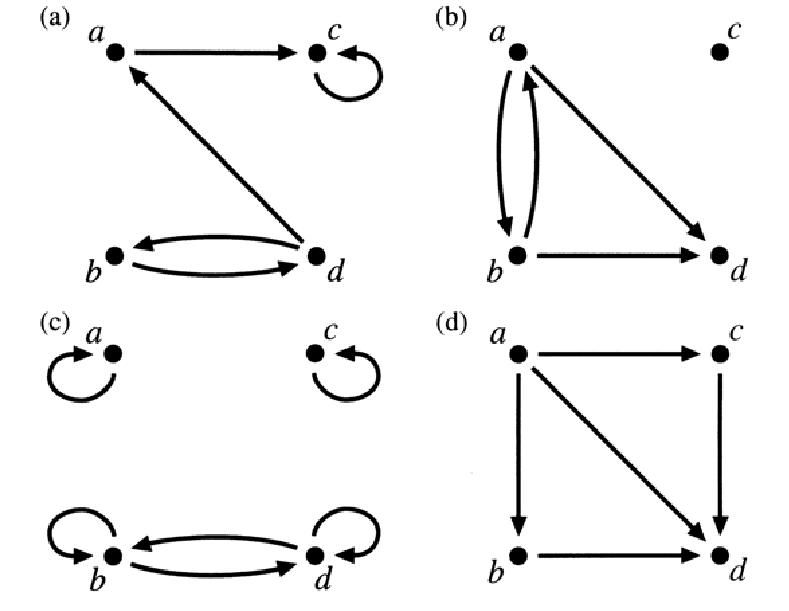
\includegraphics[width=0.5\textwidth]{images/4.3_4.png} 
\end{figure}

\textbf{Solution (a):}

\[R = \{(a, c), (d, a), (d, b), (b, d)\}\]
Reflexive: NO, Symmetric: NO, Transitive: NO

\textbf{Solution (b):}

\[R = \{(a, d), (b, d), (b, a), (a, b)\}\]
Reflexive: NO, Symmetric: NO, Transitive: NO

\textbf{Solution (c):}

\[R = \{(a, a), (b, b), (c, c), (d, d), (b, d), (d, b)\}\]
Reflexive: YES, Symmetric: YES, Transitive: YES

\textbf{Solution (d):}

\[R = \{(a, c), (a, b), (a, d), (b, d), (c, d)\}\]
Reflexive: NO, Symmetric: NO, Transitive: YES

\begin{tcolorbox}[title=Problem 5, breakable]
    Figure $4.5$ shows two relations $R$ and $S$. Find $S \circ R$.
\end{tcolorbox}

\begin{figure}[h] 
\centering
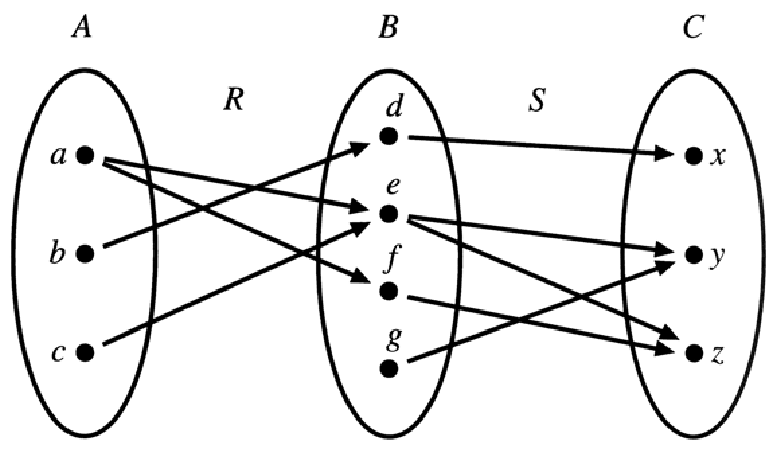
\includegraphics[width=0.5\textwidth]{images/4.3_5.png} 
\end{figure}

\textbf{Solution:}

$S \circ R = \{(a, y), (a, z), (a, z), (b, x), (c, y), (c, z)\}$

\begin{tcolorbox}[title=Problem 7, breakable]
    Prove $R$ is reflexive iff $i_A \subseteq R$,
    where $i_A$ is the identity relation of $A$.
\end{tcolorbox}

\begin{proof}
    ($\rightarrow$) Suppose $R$ is reflexive.
    It follows that for all $x \in A$, $(x, x) \in R$.
    So we can select two arbitrary elements $x, y \in A$
        and if $x = y$ then $(x, y) = (x, x) \in R$.
    Therefore $i_A \subseteq R$.

    ($\leftarrow$) Suppose $i_A \subseteq R$.
    For all $x, y \in A$ where $x = y$, $(x, y) \in R$.
    So we can select two arbitrary elements $x, x \in A$
        and since $x = x$, $(x, x) \in R$.
    Therefore, $R$ is reflexive.
\end{proof}

\begin{tcolorbox}[title=Problem 8, breakable]
    Prove $R$ is transitive iff $R \circ R \subset R$.
\end{tcolorbox}

\begin{proof}
    ($\rightarrow$) Suppose $R$ is transitive.
    So for all $x, y, z \in A$, if $(x, y) \in R$ 
        and $(y, z) \in R$ then $(x, z) \in R$.
    Let $(x, y)$ be an arbitrary pair of elements in $R \circ R$.
    There exists an element $c$ such that $(x, c) \in R$ and $(c, y) \in R$.
    Since $(x, c) \in R$ and $(c, y) \in R$ it follows that $(x, y) \in R$.

    ($\leftarrow$) Suppose $R \circ R \subseteq R$.
    Let $(x, y)$ be an arbitrary pair of elements in $R \circ R$.
    There exists an element $c$ such that $(x, c) \in R$ and $(c, y) \in R$.
    It follows since $R \circ R \subseteq R$ that $(x, y) \in R$.
    Since $(x, y)$ was arbitrary in $R \circ R$, this holds 
        for all $x, y, z \in A$. 
    So if $(x, z) \in R$ and $(z, y) \in R$, then $(x, y) \in R$.
    Therefore, $R$ is transitive.
\end{proof}

\begin{tcolorbox}[title=Problem 9, breakable]
    Suppose $A$ and $B$ are sets.

    (a) Show that for every relation $R$ from $A$ to $B$. $R \circ i_A = R$.

    (b) Show that for every relation $R$ from $A$ to $B$. $i_B \circ R = R$.
\end{tcolorbox}

\begin{proof}
    We first show $R \circ i_A \subseteq R$.
    Let $(x, y)$ be an arbitrary pair of elements in $R \circ i_A$.
    There exists an element $c$ such that $(x, c) \in i_A$ and $(c, y) \in R$.
    But $(x, c) \in i_A$ so $c = x$.
    Therefore $(x, y) \in R$.

    We now show $R \subseteq R \circ i_A$.
    Let $(x, y)$ be an arbitrary pair of elements in $R$.
    We know $(x, x) \in i_A$. 
    Since $(x, x) \in i_A$ and $(x, y) \in R$, $(x, y) \in R \circ i_A$.

    Since $R \circ i_A \subseteq R$ and $R \subseteq R \circ i_A$
        $R \circ i_A = R$.
\end{proof}

\begin{proof}
    We first show $i_B \circ R \subseteq R$.
    Let $(x, y)$ be an arbitrary pair of elements in $i_B \circ R$.
    There exists an element $c$ such that $(x, c) \in R$ and $(c, y) \in i_B$.
    Since $(c, y) \in i_B$, $y = c$.
    Therefore $(x, y) \in R$.

    We now show $R \subseteq i_B \circ R$.
    Let $(x, y)$ be an arbitrary pair of elements in $R$.
    We know $(y, y) \in i_B$.
    Since $(x, y) \in R$ and $(y, y) \in i_B$, $(x, y) \in i_B \circ R$.

    Since $i_B \circ R \subseteq R$ and $R \subseteq i_B \circ R$,
        $i_B \circ R = R$.
\end{proof}

\begin{tcolorbox}[title=Problem 10, breakable]
    Suppose $S$ is a relation on $A$.
    Let $D = Dom(S)$ and $R = Ran(S)$.

    Prove that $i_D \subseteq S^{-1} \circ S$
        and $i_R \subseteq S \circ S^{-1}$.

    Prove that $i_R \subseteq S \circ S^{-1}$.
\end{tcolorbox}

\begin{proof}
    Let $(x, x)$ be an arbitrary pair in $i_D$.
    There exists $y$ such that $(x, y) \in S$.
    Clearly $(y, x) \in S^{-1}$.
    Since $(x, y) \in S$ and $(y, x) \in S^{-1}$ 
        then $(x, x) \in S \circ S^{-1}$.
\end{proof}

\begin{proof}
    Let $(y, y)$ be an arbitrary pair in $i_R$.
    There exists $x$ such that $(x, y) \in S$.
    Clearly $(y, x) \in S^{-1}$.
    Since $(x, y) \in S$ and $(y, x) \in S^{-1}$ 
        then $(y, y) \in S \circ S^{-1}$.
\end{proof}

\begin{tcolorbox}[title=Problem 11, breakable]
    Suppose $R$ is a relation on $A$.
    Prove that if $R$ is reflexive then $R \subseteq R \circ R$.
\end{tcolorbox}

\begin{proof}
    Suppose $R$ is reflexive.
    Let $(x, y)$ be an arbitrary pair in $R$.
    Since $R$ is reflexive $(y, y) \in R$.
    Let $z = y$, then $(x, z) \in R$ and $(z, y) \in R$.
    Therefore $(x, y) \in R \circ R$.
\end{proof}

\begin{tcolorbox}[title=Problem 12, breakable]
    Suppose $R$ is a relation on $A$.

    (a) Prove that if $R$ is reflexive, then so is $R^{-1}$

    (b) Prove that if $R$ is symmetric, then so is $R^{-1}$.

    (c) Prove that if $R$ is transitive, then so is $R^{-1}$.
\end{tcolorbox}

\begin{proof}
    Suppose $R$ is reflexive.
    Let $x$ be an arbitrary element in $A$.
    Since $R$ is reflexive $(x, x) \in R$.
    Since $(x, x) \in R$, $(x, x) \in R^{-1}$.
    Since for all $x \in A$, $(x, x) \in R^{-1}$ it follows that $R^{-1}$ is reflexive.
\end{proof}

\begin{proof}
    Suppose $R$ is symmetric.
    Let $x, y$ be elements in $A$ such that $(x, y) \in R$.
    Since $R$ is symmetric $(y, x) \in R$.
    Since $(x, y) \in R$ then $(y, x) \in R^{-1}$.
    Since $(y, x) \in R$ then $(x, y) \in R^{-1}$.
    Since $(y, x) \in R^{-1}$ and $(x, y) \in R^{-1}$ it follows that
        $R^{-1}$ is symmetric.
\end{proof}

\begin{proof}
    Suppose $R$ is transitive.
    Let $x, y, z$ be arbitrary elements in A such that $(x, y) \in R$
    and $(y, z) \in R$. Since $R$ is transitive $(x, z) \in R$.
    Clearly, $(y, x) \in R^{-1}$, $(z, y) \in R^{-1}$, and $(z, x) \in R^{-1}$.
    Since $(z, x), (z, y), (y, x)\in R^{-1}$ it follows that
        $R^{-1}$ is transitive.
\end{proof}

\begin{tcolorbox}[title=Problem 12, breakable]
    Suppose $R$ is a relation on $A$.

    (a) Prove that if $R$ is reflexive, then so is $R^{-1}$.

    (b) Prove that if $R$ is symmetric, then so is $R^{-1}$.

    (c) Prove that if $R$ is transitive, then so is $R^{-1}$.
\end{tcolorbox}

\begin{proof}    
    Suppose $R$ is reflexive.
    Let $x$ be an arbitrary element in $A$.
    Since $R$ is reflexive $(x, x) \in R$.
    It then follows trivially that $(x, x) \in R^{-1}$.
    Therefore $R^{-1}$ is reflexive.
\end{proof}

\begin{proof}
    Suppose $R$ is symmetric.
    Let $(y, x)$ be an arbitrary element in $R^{-1}$.
    It follows that $(x, y) \in R$.
    Since $R$ is symmetric $(y, x) \in R$.
    It follows that $(x, y) \in R^{-1}$.
    Therefore $R^{-1}$ is symmetric.
\end{proof}

\begin{proof}
    Suppose $R$ is transitive.
    Let $(x, y)$ and $(y, z)$ be arbitrary elements in $R^{-1}$.
    It follows that $(y, x) \in R$ and $(z, y) \in R$.
    Since $R$ is transitive $(z, x) \in R$.
    It follows that $(x, z) \in R^{-1}$.
    Therefore $R^{-1}$ is transitive. 
\end{proof}

\begin{tcolorbox}[title=Problem 13, breakable]
    Suppose $R_1$ and $R_2$ are relations on $A$.
    For each part give either a proof or a counterexample to justify your answer.

    (a) If $R_1$ and $R_2$ are reflexive, must $R_1 \cup R_2$ be reflexive?

    (b) If $R_1$ and $R_2$ are symmetric, must $R_1 \cup R_2$ be symmetric?

    (c) If $R_1$ and $R_2$ are transitive, must $R_1 \cup R_2$ be transitive?
\end{tcolorbox}

\begin{proof}
    Suppose $R_1$ and $R_2$ are reflexive.
    Let $x$ be an arbitrary element in $A$.
    Since $R_1$ and $R_2$ are reflexive it follows that $(x, x) \in R_1$ and $(x, x) \in R_2$.
    It follows that $(x, x) \in R_1 \cup R_2$.
    Therefore $R_1 \cup R_2$ is reflexive.
\end{proof}

\begin{proof}
    Suppose $R_1$ and $R_2$ are symmetric.
    Let $(x, y)$ be an arbitrary element in $R_1 \cup R_2$.
    It follows that $(x, y) \in R_1$ or $(x, y) \in R_2$.
    Suppose $(x, y) \in R_1$.
    Since $R_1$ is symmetric $(y, x) \in R_1$ and therefore $(y, x) \in R_1 \cup R_2$.
    Suppose $(x, y) \in R_2$.
    Since $R_2$ is symmetric $(y, x) \in R_2$ and therefore $(y, x) \in R_1 \cup R_2$.
    Therefore $R_1 \cup R_2$ is symmetric.
\end{proof}

\textbf{Solution:}
\[A = \{1, 2, 3\} \quad R_1 = \{(1, 2)\} \quad R_2 = \{(2, 3)\}\]
\[R_1 \cup R_2 = \{(1, 2), (2, 3)\}\]
Now clearly $R_1$ and $R_2$ are transitive. However, $R_1 \cup R_2$ is not transitive because 
    $(1, 2) \in R_1 \cup R_2$ and $(2, 3) \in R_1 \cup R_2$
    but $(1, 3) \not \in R_1 \cup R_2$

\begin{tcolorbox}[title=Problem 22, breakable]
    Consider the following putative theorem:
    \begin{theorem}
        Suppose $R$ is a relation on $A$. If $R$ is symmetric and 
        transitive, then $R$ is reflexive.
    \end{theorem}
    Is the following proof correct? If so, what proof strategies does it use?
    If not, can it be fixed? Is the theorem correct?
    \begin{proof}
        Let $x$ be an arbitrary element of $A$. Let $y$ be any element of $A$
        such that $xRy$. Since $R$ is symmetric, it follows that $yRx$.
        But then by transitivity, since $xRy$ and $yRx$ we can conclude 
        that $xRx$. Since $x$ was arbitrary, we have shown that $\forall{x} \in A (xRx)$,
        so $R$ is reflexive.
    \end{proof}
\end{tcolorbox}

\textbf{Solution:}

The proof is invalid since it assumes properties about $y \in A$ namely that $x, y \in R$.
The theorem is incorrect so it cannot be fixed.

\begin{tcolorbox}[title=Problem 24, breakable]
    Let $R = \{(m, n) \in \mathbb{N} \times \mathbb{N} \mid |m - n| \le 1\}$,
    which is a relation on $\mathbb{Z}$. This exercise will illustrate
    why, in part $1$ of Definition $4.3.2$, we define the phrase ``$R$ is 
    reflexive on $A$'', rather than simply ``$R$ is reflexive''.
    
    (a) Is $R$ reflexive on $\mathbb{N}$?

    (b) Is $R$ reflexive on $\mathbb{Z}$?
\end{tcolorbox}

\textbf{Solution (a):}

Yes $R$ is reflexive on $\mathbb{N}$. Let $x$ be an arbitrary element in $\mathbb{N}$.
    It follows that $|x - x| = 0 \le 1$ and therefore $(x, x) \in R$.
    
\textbf{Solution (b):} 

Yes $R$ is reflexive on $\mathbb{Z}$. Let $x$ be an arbitrary element in $\mathbb{Z}$.
    It follows that $|x - x| = 0 \le 1$ and therefore $(x, x) \in R$.

\subsection{Ordering Relations}

\begin{tcolorbox}[title=Problem 1, breakable]
    In each case, say whether or not $R$ is a partial order on $A$.
    If so, is it a total order? 

    (a) $A = \{a, b, c\}, R = \{(a, a), (b, a), (b, b), (b, c), (c, c)\}$ 

    (b) $A = \mathbb{R}, R = \{(x, y) \in \mathbb{R} \times \mathbb{R} \mid |x| \le |y|\}$ 

    (c) $A = \mathbb{R}, R = \{(x, y) \in \mathbb{R} \times \mathbb{R} \mid |x| < |y| \text{ or } x = y\}$
\end{tcolorbox}

\textbf{Solution (a):}

$R$ is a partial order on $A$.
$R$ is not a total order on $A$ because $aRc$ and $cRa$ are false.

\textbf{Solution (b):}

$R$ is not a partial order.
Consider $(3, -3)$ so clearly $3R(-3)$ and $(-3)R3$ but $3 \not= -3$.

\textbf{Solution (c):}

$R$ is a partial order on $A$.
$R$ is not a total order because $5R(-5)$ and $(-5)R5$ are false.

\begin{tcolorbox}[title=Problem 2, breakable]
    In each case, say whether or not $R$ is a partial order on $A$. 
    If so, is it a total order? 

    (a) $A =$ the set of all English words.  
    $R = \{(x, y) \in A \times A \mid$  
    where the word $y$ occurs at least as late in alphabetical order as the word $x$$\}$.

    (b) $A =$ the set of all English words.  
    $R = \{(x, y) \in A \times A \mid$  
    where the first letter of the word $y$ occurs at least as late in the alphabet as the first letter of the word $x$$\}$.

    (c) $A =$ the set of all countries in the world.  
    $R = \{(x, y) \in A \times A \mid$  
    where the population of country $y$ is at least as large as the population of country $x$$\}$.
\end{tcolorbox}

\textbf{Solution (a):}

$R$ is a partial order on $A$ and a total order on $A$.

\textbf{Solution (b):}

$R$ is not a partial order on $A$.
Consider ``the'' and ``tip''.
Now ``the''$R$``tip'' and ``tip''$R$``the'' but ``tip''$\not= $``the''.
So $R$ is not antisymmetric.

\textbf{Solution (c)}

$R$ is not a partial order on $A$.
Consider $a =$ America population $100$ and $m =$  Mexico population $100$.
Then $aRm$ and $mRa$ but $a \not= m$ so $R$ is not antisymmetric.

\begin{tcolorbox}[title=Problem 3, breakable]
    In each case find all minimal and maximal elements of $B$.
    Also find, if they exist, the largest and smallest elements of $B$,
    and the least upper bound and greatest lower bound of $B$.

    (a) $R =$ the relation shown in the directed graph in Figure $4.6$,
        $B = \{2, 3, 4\}$.

    (b) $R = \{(x, y \in \mathbb{\mathbb{R}} \times \mathbb{\mathbb{R}} \mid x \le y)\}$,
        $B = \{(x \in \mathbb{R} \mid 1 \le x < 2)\}$.

    (c) $R = \{(x, y) \in \mathcal{P}(\mathbb{N}) \times \mathcal{P}(\mathbb{N}) \mid x \subseteq y\}$,
        $B = \{(x \in \mathcal{P}(\mathbb{N})) \mid \text{$x$ has at most $5$ elements.}\}$
\end{tcolorbox}

\begin{figure}[h] 
\centering
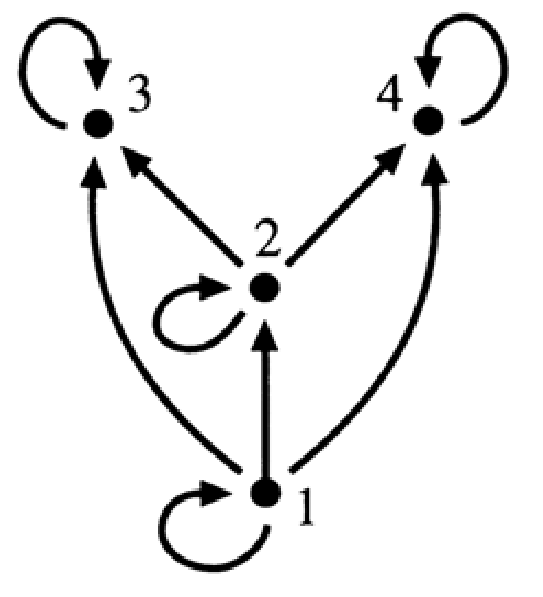
\includegraphics[width=0.3\textwidth]{images/4.4_2.png} 
\end{figure}

\textbf{Solution (a):}

Minimal elements: $\{2\}$, Maximal elements: $\{3, 4\}$

Smallest element: $2$, Largest element: none

Greatest lower bound: $2$, Least upper bound: none

\textbf{Solution (b):}

Minimal elements: $\{1\}$, Maximal elements: none

Smallest element: $1$, Largest element: none

Greatest lower bound: $1$, Least upper bound: $2$

\textbf{Solution (c):}

Minimal elements: $\{\emptyset\}$, Maximal elements: Any $5$ element subset of $\mathbb{N}$

Smallest element: $\emptyset$, Largest element: none

Greatest lower bound: $\emptyset$, Least upper bound: none

\begin{tcolorbox}[title=Problem 4, breakable]
    Suppose $R$ is a relation on $A$. You might think $R$ could not be both 
    antisymmetric and symmetric, but this isn't true. Prove that $R$ is both 
    antisymmetric and symmetric iff $R \subseteq i_A$.
\end{tcolorbox}

\begin{proof}
    ($\rightarrow$) Suppose $R$ is both antisymmetric and symmetric.
    Let $x$, $y$ be arbitrary elements in $A$ such that $xRy$.
    Since $R$ is symmetric and $xRy$ it follows that $yRx$.
    Then, since $R$ is antisymmetric and $xRy$ and $yRx$, it follows that $x = y$.
    Therefore $(x, y) = (x, x) \in i_A$.

    ($\leftarrow$) Suppose $R \subseteq i_A$.
    Let $x$, $y$ be arbitrary elements in $A$ such that $xRy$.
    Since $R \subseteq i_A$ it follows that $(x, y) \in i_A$ and therefore $x = y$.
    So $xRy$ and $yRx$ implies $x = y$ so $R$ is antisymmetric.
    Also, $xRy$ implies $yRx$ so $R$ is symmetric.

    Thus $R$ is both antisymmetric and symmetric iff $R \subseteq i_A$.
\end{proof}

\begin{tcolorbox}[title=Problem 6, breakable]
    Suppose $R_1$ and $R_2$ are partial orders on $A$.
    For each part, give either a proof or a counterexample to justify your answer.

    (a) Must $R_1 \cap R_2$ be a partial order on $A$?

    (b) Must $R_1 \cup R_2$ be a partial order on $A$?
\end{tcolorbox}

\begin{proof}
    To prove that $R_1 \cap R_2$ is a partial order on $A$,
        we must show it is reflexive, antisymmetric, and transitive on $A$.
    First note that $R_1$, $R_2$ being partial orders on $A$ implies that 
        they are reflexive, antisymmetric, and transitive on $A$.

    We first show $R_1 \cap R_2$ is reflexive.
    Let $x$ be an arbitrary element in $A$.
    Since $R_1$, $R_2$ are reflexive on $A$ it follows that $xR_1x$ and $xR_2x$.
    It then follows that $x(R_1 \cap R_2)x$.
    Therefore $R_1 \cap R_2$ is reflexive.

    We now show $R_1 \cap R_2$ is antisymmetric.
    Let $x$, $y$ be arbitrary elements in $A$ such that $x(R_1 \cap R_2)y$
        and $y(R_1 \cap R_2)x$.
    This implies $xR_1y$ and $yR_1x$.
    Since $R_1$ is antisymmetric it follows that $y = x$.
    A similar argument shows $y = x$ on $R_2$.
    Therefore $R_1 \cap R_2$ is antisymmetric.

    Finally, we show $R_1 \cap R_2$ is transitive.
    Suppose $x$, $y$, $z$ are arbitrary elements in $A$ such that $x(R_1 \cap R_2)y$
        and $y(R_1 \cap R_2)z$.
    It follows that $xR_1y$ and $yR_1z$.
    Since $R_1$ is transitive it follows that $xR_1z$.
    A similar argument shows $xR_2z$.
    Therefore $R_1 \cap R_2$ is transitive.

    Since $R_1 \cap R_2$ is reflexive, antisymmetric, and transitive,
         it is a partial order on $A$.
\end{proof}

\textbf{Solution (b):}

\[A = \{1, 2, 3\} \quad R_1 = \{(1, 1), (2, 2), (3, 3), (1, 2)\} \quad R_2 = \{(1, 1), (2, 2), (3, 3) (2, 3)\}\]
\[R_1 \cup R_2 = \{(1, 1), (2, 2), (3, 3), (1, 2), (2, 3)\}\]

Notice $1(R_1 \cup R_2)2$ and $2(R_1 \cup R_2)3$ but not $1(R_1 \cup R_2)3$
    therefore $R_1 \cup R_2$ is not transitive and not a partial order.

\begin{tcolorbox}[title=Problem 13, breakable]
    Suppose $R$ is a partial order on $A$. Prove that $R^{-1}$
    is also a partial order on $A$. If $R$ is a total order,
    will $R^{-1}$ also be a total order?
\end{tcolorbox}

\begin{proof}
    Suppose $R$ is a partial order on $A$.

    Let $x$ be an arbitrary element in $A$.
    Since $R$ is a partial order it is reflexive therefore $xRx$.
    But $xRx$ implies $xR^{-1}x$ so $R^{-1}$ is reflexive.

    Let $x$, $y$ be arbitrary elements in $A$ such that $xR^{-1}y$ and $yR^{-1}x$.
    Since $xR^{-1}y$, $yR^{-1}x$ it follows that $yRx$, $xRy$.
    Since $R$ is a partial order it is antisymmetric therefore since $yRx$, $xRy$
        it follows that $x = y$.
    Thus $xR^{-1}y$ and $yR^{-1}x$ implies $x = y$ so $R^{-1}$ is antisymmetric.

    Let $x$, $y$, $z$ be arbitrary elements in $A$ such that $xR^{-1}y$ and $yR^{-1}z$.
    Since $xR^{-1}y$, $yR^{-1}z$ it follows that $yRx$, $zRy$.
    Since $R$ is a partial order it is transitive therefore since $zRy$, $yRx$
        it follows that $zRx$ and therefore $xR^{-1}z$.
    Thus $xR^{-1}y$ and $yR^{-1}z$ implies $xR^{-1}z$ so $R^{-1}$ is transitive.

    Since $R^{-1}$ was reflexive, antisymmetric, and transitive it is a partial order.
\end{proof}

\textbf{Solution (b):}

By the previous proof if $R$ is a total order than $R^{-1}$ is at least a partial order.
Now, $R$ being a total order implies for all $x$, $y$ either $xRy$ or $yRx$.
Clearly either $yR^{-1}x$ or $xR^{-1}y$ is true in that case therefore $R^{-1}$ is 
also a total order.

\begin{tcolorbox}[title=Problem 14, breakable]
    Suppose $R$ is a partial order on $A$, $B \subseteq A$, and $b \in B$.
    exercise $13$ shows that $R^{-1}$ is also a partial order on $A$.

    (a) Prove that $b$ is the $R$-largest element of $B$ iff it is the $R^{-1}$-smallest
        element of $B$.

    (b) Prove that $b$ is an $R$-maximal element of $B$ iff it is an $R^{-1}$-minimal 
        element of $B$.
\end{tcolorbox}

\begin{proof}
    ($\rightarrow$) Suppose that $b$ is an $R$-largest element of $B$.
    So for all $a \in B$, $aRb$. 
    It then follows that $bR^{-1}a$.
    Since $a$ was arbitrary, for all $a \in B$, $bR^{-1}a$. 
    So $b$ is the $R^{-1}$-smallest element of $B$.

    ($\leftarrow$) The argument is symmetrical.

    Therefore $b$ is the $R$-largest element of $B$ iff it is the $R^{-1}$-smallest
        element of $B$.
\end{proof}

\begin{proof}
    ($\rightarrow$) Suppose that $b$ is an $R$-maximal element of $B$.
    There does not exist $a \in B$ such that $bRa$ and $b \not= a$.
    So there does not exist $a \in B$ such that $aR^{-1}b$ and $a \not= b$.
    Therefore $b$ is the $R^{-1}$-minimal element of $B$.

    ($\leftarrow$) The argument is symmetrical.

    Therefore $b$ is an $R$-maximal element of $B$ iff it is an $R^{-1}$-minimal 
        element of $B$.
\end{proof}

\begin{tcolorbox}[title=Problem 19, breakable]
    Consider the following putative theorem. \\

    \textbf{Theorem} Suppose $R$ is a total order on $A$ and $B \subset A$.
    Then every element of $B$ is either the smallest element of $B$
    or the largest element of $B$. \\

    (a) What's wrong with the following proof of the theorem? \\
    \begin{proof}
        Suppose $b \in B$. Let $x$ be an arbitrary element of $B$.
        Since $R$ is a total order, either $bRx$ or $xRb$.

        Case $1$. $bRx$. Since $x$ was arbitrary, we can conclude that 
        $\forall{x} \in B(bRx)$, so $b$ is the smallest element of $R$.

        Case $2$. $xRb$. Since $x$ was arbitrary, we can conclude that 
        $\forall{x} \in B(xRb)$, so $b$ is the largest element of $R$.

        Thus, $b$ is either the smallest element of $B$ or the largest element 
        of $B$. Since $b$ was arbitrary, every element of $B$ is either its 
        smallest element or its largest element.
    \end{proof}

    (b) Is the theorem correct? Justify your answer with either a proof 
        or a counterexample.
\end{tcolorbox}

\textbf{Solution (a):}

Within each case $x$ is not an arbitrary element of $B$.
The issue is $x$ has an additional property that $bRx$ in case $1$
and $xRb$ in case $2$.

\textbf{Solution (b):}

The theorem is incorrect. Consider the following counterexample:
\[A = \mathbb{N}, B = \{1, 2, 3\}, R = \{(x, y) \in A \times A \mid x \le y\}\]
Clearly $2$ is not the R-largest element since $(2, 3) \in R$ and $2 \not= 3$.
But $2$ is also not the R-smallest element since $(1, 2) \in R$ and $1 \not= 2$.

\begin{tcolorbox}[title=Problem 23, breakable]
    Prove Theorem $4.4.11$.

    \textbf{Theorem $4.4.11$} Suppose $A$ is a set $\mathcal{F} \subseteq \mathcal{P}(A)$,
    and $\mathcal{F} \not= \emptyset$. Then the least upper 
    bound of $\mathcal{F}$ (in the subset partial order) is $\bigcup\mathcal{F}$
    and the greatest lower bound of $\mathcal{F}$ is $\bigcap\mathcal{F}$.
\end{tcolorbox}

\begin{proof}
    Let $y$ be an arbitrary element in $A$ such that $A \in \mathcal{F}$.
    For all $x \in B$ where $B \in \mathcal{F}$, $x \in \bigcup \mathcal{F}$.
    Since $y \in A$ where $A \in \mathcal{F}$, $y \in \bigcup \mathcal{F}$. 
    Thus $\bigcup \mathcal{F}$ is an upper bound.
    Now, suppose there exists a smaller upper bound $\mathcal{G}$ such that $\mathcal{G} \subset \bigcup \mathcal{F}$.
    Let $x$ be an element in $\bigcup \mathcal{F}$ that is not in $\mathcal{G}$. 
    Then $x \in A$ for some $A \in \mathcal{F}$, but $x \notin \mathcal{G}$, so $A \not\subseteq \mathcal{G}$.
    So $\mathcal{G}$ is not an upper bound.
    Thus $\bigcup \mathcal{F}$ is the \emph{l.u.b}.
\end{proof}

\begin{proof}
    Let $y$ be an arbitrary element in $A$ such that $A \in \mathcal{F}$.
    For all $x \in \bigcap \mathcal{F}$, we have $x \in B$ for every $B \in \mathcal{F}$.
    Thus $\bigcap \mathcal{F} \subseteq A$ for all $A \in \mathcal{F}$,
        which shows that $\bigcap \mathcal{F}$ is a lower bound.
    Now, suppose there exists a greater lower bound $\mathcal{G}$ such that 
    $\bigcap \mathcal{F} \subset \mathcal{G}$.
    Let $x$ be an element in $\mathcal{G}$ that is not in $\bigcap \mathcal{F}$.
    Then $x \notin A$ for some $A \in \mathcal{F}$, so $\mathcal{G} \not\subseteq A$.
    So $\mathcal{G}$ is not a lower bound.
    Thus $\bigcap \mathcal{F}$ is the \emph{g.l.b}.
\end{proof}

\begin{tcolorbox}[title=Problem 24, breakable]
    Suppose $R$ is a relation on $A$. Let $S = R \cup R^{-1}$.

    (a) Show that $S$ is a symmetric relation on $A$ and $R \subseteq S$.

    (b) Show that if $T$ is symmetric relation on $A$ and $R \subseteq T$
        then $S \subseteq T$.

    Note that this exercise shows that $S$ is the smallest element of the set 
    $\mathcal{F} = \{T \subseteq A \times A \mid R \subseteq T \text{ and } T \textbf{ is symmetric}\}$;
    in other words, it is the smallest symmetric relation on $A$ that contains $R$ as a subset. This 
    relation $S$ is called the symmetric closure of $R$.
\end{tcolorbox}

\begin{proof}
    Suppose $x, y$ are arbitrary elements in $A$ and $(x, y) \in S$.
    So $(x, y) \in R \cup R^{-1}$.
    Thefore $(x, y) \in R$ or $(x, y) \in R^{-1}$.
    Suppose $(x, y) \in R$ then $(y, x) \in R^{-1}$
        and it follows that $(y, x) \in R \cup R^{-1} = S$.
    Suppose $(x, y) \in R^{-1}$ then $(y, x) \in R$
        and it follows that $(y, x) \in R \cup R^{-1} = S$.
    Therefore $S$ is a symmetric relation on $A$.
\end{proof}

\begin{proof}
    Let $(x, y)$ be an arbitrary element in $R$.
    Cearly, $(x, y) \in R \cup R^{-1} = S$.
    Therefore $R \subseteq S$.
\end{proof}

\begin{proof}
    Suppose $(x, y)$ is an arbitrary pair of elements in $S$.
    It follows that $(x, y) \in R \cup R^{-1}$.
    So $(x, y) \in R$ or $(x, y) \in R^{-1}$.
    Suppose $(x, y) \in R$.
    Since $R \subseteq T$ then $(x, y) \in T$.
    Suppose $(x, y) \in R^{-1}$ so $(y, x) \in R$.
    Since $R \subseteq T$ then $(y, x) \in T$.
    Since $T$ is symmetric it follows that $(x, y) \in T$.
    Therefore $S \subseteq T$.
\end{proof}

\begin{tcolorbox}[title=Problem 25, breakable]
    Suppose that $R$ is a relation on $A$. Let $\mathcal{F} = \{T \subseteq A \times A \mid R \subseteq T
    \text{ and } T \text{ is transitive}\}$.

    (a) Show that $\mathcal{F} \not = \emptyset$.

    (b) Show that $\bigcap \mathcal{F}$ is a transitive relation on $A$ and $R \subseteq \bigcap \mathcal{F}$.
    
    (c) Show that $\bigcap \mathcal{F}$ is the smallest transitive relation on $A$ that contains $R$ 
        as a subset. The relation $\bigcap \mathcal{F}$ is called the transitive closure of $R$.
\end{tcolorbox}

\begin{proof}
    Since $A \times A$ is a relation on $A$, $R \subseteq A \times A$, and $A \times A$ is transitive
        it follows that $A \times A \in \mathcal{F}$.
    Therefore $\mathcal{F} \not = \emptyset$. 
\end{proof}

\begin{proof}
    Suppose $(x, y)$ and $(y, z)$ are arbitrary elements in $\bigcap \mathcal{F}$.
    For all $\mathcal{G} \in \mathcal{F}$, $(x, y) \in \mathcal{G}$ and $(y, z) \in \mathcal{G}$.
    Since $\mathcal{G}$ is transitive then $(x, z) \in \mathcal{G}$.
    Since $\mathcal{G}$ was arbitrary it follows that $(x, z) \in \bigcap \mathcal{F}$.
\end{proof}

\begin{proof}
    Suppose $(x, y)$ is an arbitrary element in $R$, 
        and $\mathcal{G}$ is an arbitrary set in $\mathcal{F}$.
    Since $R \subseteq \mathcal{G}$ it follows that $(x, y) \in \mathcal{G}$.
    Since $\mathcal{G}$ was arbitrary, $(x, y) \in \bigcap \mathcal{F}$.
\end{proof}

\begin{proof}
    Suppose $(x, y)$ is an arbitrary element in $\bigcap \mathcal{F}$,
        and $T$ is a transitive relation on $A$ such that $R \subseteq T$.
    Now for all $\mathcal{G} \in \mathcal{F}$, $(x, y) \in \mathcal{G}$.
    It then follows, since $T \in \mathcal{F}$ that $(x, y) \in T$.
    Therefore $\bigcap \mathcal{F} \subseteq T$.
    Showing that $\bigcap \mathcal{F}$ is the 
        smallest transitive relation on $A$ that contains $R$ 
        as a subset.
\end{proof}

\begin{tcolorbox}[title=Problem 26, breakable]
    Suppose $R_1$ and $R_2$ are relations on $A$, and let $R_1 \subseteq R_2$.

    (a) Let $S_1$ and $S_2$ be the symmetric closures of $R_1$ and $R_2$,
        respectively. Prove that $S_1 \subseteq S_2$. (See exercise $24$ for the 
        definition of symmetric closure.)

    (b) Let $T_1$ and $T_2$ be the transitive closures of $R_1$ and $R_2$, respectively.
        Prove that $T_1 \subseteq T_2$. (See exercise $25$ for the definition of transitive
        closure.)
\end{tcolorbox}

\begin{proof}
    Let $(x, y)$ be an arbitrary element in $S_1$.
    So $(x, y) \in R_1 \cup R_1^{-1}$ therefore $(x, y) \in R_1$ or $(x, y) \in R_1^{-1}$.
    Suppose $(x, y) \in R_1$. Since $R_1 \subseteq R_2$, $(x, y) \in R_2$.
    Then $(x, y) \in R_2 \subseteq R_2 \cup R_2^{-1} = S_2$.
    Suppose $(x, y) \in R_1^{-1}$ it follows that $(y, x) \in R_1$.
    Since $R_1 \subseteq R_2$, $(y, x) \in R_2$ so $(x, y) \in R_2^{-1}$.
    Then $(x, y) \in R_2 \cup R_2^{-1} = S_2$.
    Therefore $S_1 \subseteq S_2$.
\end{proof}

\begin{proof}
    Suppose $(x, y)$ is an arbitrary element in $R_1$.
    Since $R_1 \subseteq R_2$ it follows that $(x, y) \in R_2$.
    Thus $(x, y) \in T_2$ and $R_1 \subseteq T_2$.
    Suppose $(x, y), (y, z)$ are arbitrary pairs in $R_1$.
    Since $R_1 \subseteq R_2$ it follows that $(x, y), (y, z) \in R_2$.
    Thus $(x, y), (y, z), (x, z) \in T_2$.
    So $T_2$ is a transitive relation containing $R_1$.
    Since $T_1$ is the minimal transitive relation containing $R_1$,
        it follows that $T_1 \subseteq T_2$.
\end{proof}

\begin{tcolorbox}[title=Problem 27, breakable]
    Suppose $R_1$ and $R_2$ are relations on $A$, and let $R = R_1 \cup R_2$.

    (a) Let $S_1$, $S_2$, and $S$ be symmetric closures of $R_1$, $R_2$, and $R$,
        respectively. Prove that $S_1 \cup S_2 = S$. (See exercise $24$ for the definition
        of symmetric closure.)

    (b) Let $T_1$, $T_2$, and $T$ be the transitive closures of $R_1$, $R_2$, and $R$,
        respectively. Prove that $T_1 \cup T_2 \subseteq T$, and give an example to 
        show that it may happen that $T_1 \cup T_2 \not= T$. (See exercise $25$ for 
        the definition of transitive closure.)
\end{tcolorbox}

\begin{proof}
    We first show $S_1 \cup S_2 \subseteq S$.
    Suppose $(x, y)$ is an arbitrary pair of elements in $S_1 \cup S_2$.
    So $(x, y) \in S_1$ or $(x, y) \in S_2$.

    Suppose $(x, y) \in S_1$
    So $(x, y) \in R_1 \cup R_1^{-1}$ and therefore $(x, y) \in R_1$ or $(x, y) \in R_1^{-1}$.
    Suppose $(x, y) \in R_1$ then it follows, since $R = R_1 \cup R_2$,
        $(x, y) \in R$
    Then since $S = R \cup R^{-1}$ it follows that $(x, y) \in S$.
    A similar argument shows that supposing $(x, y) \in R_1^{-1}$ then $(x, y) \in S$.
    A similar argument shows that supposing $(x, y) \in S_2$ then $(x, y) \in S$.
    Therefore $S_1 \cup S_2 \subseteq S$.

    We now show $S \subseteq S_1 \cup S_2$.
    Suppose $(x, y)$ is an arbitrary pair of elements in $S$.
    So $(x, y) \in R$ or $(x, y) \in R^{-1}$.
    Suppose $(x, y) \in R$.
    Since $R = R_1 \cup R_2$ it follows that
        $(x, y) \in R_1 \cup R_2$.
    So $(x, y) \in R_1$ or $(x, y) \in R_2$.
    Suppose $(x, y) \in R_1$ then $(x, y) \in R_1 \cup R_1^{-1} = S_1 \subseteq S_1 \cup S_2$.
    A similar argument shows that supposing $(x, y) \in R_2$
        then $(x, y) \in S_1 \cup S_2$.
    A similar argument shows that supposing $(x, y) \in R^{-1}$
        then $(x, y) \in S_1 \cup S_2$.
    Therefore $S \subseteq S_1 \cup S_2$.

    Since $S_1 \cup S_2 \subseteq S$ and $S \subseteq S_1 \cup S_2$ 
        it follows that $S = S_1 \cup S_2$.
\end{proof}

\begin{proof}
    Let $(x, y)$ be an arbitrary pair in $T_1 \cup T_2$.
    Either $(x, y) \in T_1$ or $(x, y) \in T_2$.

    Suppose $(x, y) \in R_1$.
    Since $R = R_1 \cup R_2$ it follows that $(x, y) \in R$.
    Then since $R \subseteq T$ it follows that $(x, y) \in T$.
    Thus $R_1 \subseteq T$.

    Suppose $(x, y), (y, z) \in R_1$.
    Since $R = R_1 \cup R_2$ it follows that $(x, y), (y, z) \in R$.
    Then since $T$ is the transitive closure of $R$, it follows that $(x, z) \in T$.
    Thus $T$ is a transitive relation containing $R_1$.
    Since $T_1$ is the transitive closure of $R_1$ it follows that $T_1 \subseteq T$.
    Clearly $T_1 \cup T_2 \subseteq T$.

    A similar argument shows that supposing $(x, y) \in R_2$
    then $T_1 \cup T_2 \subseteq T$.

    Therefore $T_1 \cup T_2 \subseteq T$.
\end{proof}

\textbf{Solution:}
\[R_1 = \{(3, 4)\}, R_2 = \{(4, 5)\}, R = \{(3, 4), (4, 5)\}\]
\[T_1 = \{(3, 4)\}, T_2 = \{(4, 5)\}, T_1 \cup T_2 = \{(3, 4), (4, 5)\}, T = \{(3, 4), (4, 5), (3, 5)\}\]
Clearly $T_1 \cup T_2 \ne T$.

\begin{tcolorbox}[title=Problem 28, breakable]
    Suppose $A$ is a set.

    (a) Prove that if $A$ has at least two elements then there is no largest antisymmetric
        relation on $A$. In other words, there is no relation $R$ on $A$ such that 
        $R$ is antisymmetric, and for every antisymmetric relation $S$ on $A$, $S \subseteq R$.

    (b) Suppose $R$ is a total order on $A$. Prove that $R$ is a maximal antisymmetric relation 
        on $A$. In other words, there is no antisymmetric relation $S$ on $A$ such that $R \subseteq S$
        and $R \not= S$.
\end{tcolorbox}

\begin{proof}
    Suppose $A$ has at least two elements. 
    Let $R$ be an arbitrary antisymmetric relation on $A$.
    Let $a, b \in A$ such that $a \not = b$. If $\neg aRb$ and $\neg bRa$ then we 
    can construct a relation $S$ such that $S = R \cup \{(a, b)\}$ or $S = R \cup \{(b, a)\}$.
    In either case $S \not\subseteq R$. So either $aRb$ or $bRa$.
    Suppose $aRb$. Then we can construct a relation $S$ such that 
    $S = (R \setminus \{(a, b)\}) \cup \{(b, a)\}$;
        then $S \not\subseteq R$.
    Suppose $bRa$. Then we can construct a relation $S$ such that 
    $S = (R \setminus \{(b, a)\}) \cup \{(a, b)\}$;
        then $S \not\subseteq R$.
    Therefore there is no largest antisymmetric relation on $A$.
\end{proof}

\begin{proof}
    Suppose $S$ is an antisymmetric relation on $A$ such that 
        $R \subseteq S$ and $R \not = S$.
    Let $(a, b)$ be a pair of elements such that $(a, b) \in S$
        and $(a, b) \not \in R$.
    Since $R$ is a total order and $(a,b) \notin R$, it follows that $a \not = b$
        and $(b, a) \in R$.
    Since $(a, b) \in S$ and $a \not = b$ it follows that $(b, a) \not \in S$.
    Finally, $(b, a) \in R$ and $(b, a) \not \in S$ contradicts that $R \subseteq S$.
    Thus $R$ is a maximal antisymmetric relation on $A$.
\end{proof}

\begin{tcolorbox}[title=Problem 30, breakable]
    Suppose $R$ is a relation on $A$, and let $T$ be the transitive closure of $R$.
    Prove that if $R$ is symmetric, then so is $T$. (Hint: Assume that $R$ is symmetric.
    Prove that $R \subseteq T^{-1}$ and $T^{-1}$ is transitive. What can you conclude 
    about $T$ and $T^{-1}$? See exercise $25$ for the definition of transitive closure.)
\end{tcolorbox}

\begin{proof}
    Suppose $R$ is symmetric. Let $(x, y)$ be an arbitrary element in $R$.
    Since $R$ is symmetric it follows that $(y, x) \in R$.
    Then $(y, x) \in T$ so $(x, y) \in T^{-1}$.
    Therefore $R \subseteq T^{-1}$.

    Suppose $(x, y), (y, z)$ are arbitrary pairs in $T^{-1}$.
    It follows that $(y, x), (z, y) \in T$.
    Then, since $T$ is transitive, $(z, x) \in T$ so $(x, z) \in T^{-1}$.
    Therefore $T^{-1}$ is transitive and contains $R$.

    Now, since $R \subseteq T^{-1}$ and $T^{-1}$ is transitive, 
    $T$, being the minimal transitive closure of $R$, thus $T \subseteq T^{-1}$.

    Let $U$ be any transitive relation containing $R$.
    Then $U^{-1}$ is transitive and contains $R$, so by minimality of $T$, $T \subseteq U^{-1}$.
    Taking inverses gives $T^{-1} \subseteq U$.
    Since $U$ was arbitrary, $T^{-1}$ is minimal.
    Thus $T^{-1} = T$, showing that $T$ is symmetric.
\end{proof}

\subsection{Equivalence Relations}

\begin{tcolorbox}[title=Problem 1, breakable]
    Find all partitions of the set $A = \{1, 2, 3\}$
\end{tcolorbox}

\textbf{Solution:}

$\mathcal{F}$ is a partition of $A$ if it has the following properites:
\begin{enumerate}
    \item $\bigcup \mathcal{F} = A$.
    \item $\mathcal{F}$ is pairwise disjoint.
    \item $\forall{X \in \mathcal{F}}(X \not = \emptyset)$.
\end{enumerate}

Partitions of $A$:
\begin{enumerate}
    \item $\{\{1\}, \{2\}, \{3\}\}$
    \item $\{\{1, 2\}, \{3\}\}$
    \item $\{\{1\}, \{2, 3\}\}$
    \item $\{\{1, 3\}, \{2\}\}$
    \item $\{\{1, 2, 3\}\}$
\end{enumerate}

\begin{tcolorbox}[title=Problem 2, breakable]
    Find all equivalence relations on the set $A = \{1, 2, 3\}$.
\end{tcolorbox}

\textbf{Solution:}

$R$ is called an equivalence relation on $A$ if it is reflexive,
    symmetric, and transitive.

All equivalence relations on $A$:
\begin{enumerate}
    \item \{(1, 1), (2, 2), (3, 3)\}
    \item \{(1, 1), (2, 2), (3, 3), (1, 2), (2, 1)\}
    \item \{(1, 1), (2, 2), (3, 3), (2, 3), (3, 2)\}
    \item \{(1, 1), (2, 2), (3, 3), (1, 3), (3, 1)\}
    \item \{(1, 1), (2, 2), (3, 3), (1, 2), (2, 1), (1, 3), (3, 1), (2, 3), (3, 2)\}
\end{enumerate}

\begin{tcolorbox}[title=Problem 7, breakable]
    Let $T$ be the set of all triangles, and let 
        $S = \{(s, t) \in T \times T \mid \text{the triangles $s$ and $t$ are similar}\}$.
    (Recall that two triangles are similar if the angles of one triangle are equal to 
        corresponding angles of the other.) Verify that $S$ is an equivalent relation.
\end{tcolorbox}

\begin{proof}
    We need to show $S$ is reflexive, symmetric, and transitive.
    Clearly a triangle is similar to itself so $S$ is reflexive.
    Also, given two triangles $A, B$ if $A$ is similar to $B$ then $B$ is similar to $A$
        thus $S$ is symmetric.
    Finally, given three triangles $A, B, C$ if $A$ is similar to $B$ and $B$ is similar to 
        $C$ then $A$ is similar to $C$ thus $S$ is transitive.
    Therefore $S$ is an equivalence relation on $T$.
\end{proof}

\begin{tcolorbox}[title=Problem 8, breakable]
    Complete the proof of Lemma $4.5.7$.

    We'll prove that $R$ is reflexive and leave the rest for you 
        to do in excersize $8$.
\end{tcolorbox}

\begin{lemma}
    Suppose $A$ is a set and $\mathcal{F}$ is a partition of $A$.
    Let $R = \bigcup_{X \in \mathcal{F}}(X \times X)$.
    Then $R$ is an equivalence relation on $A$.
    We will call $R$ the equivalence relation determined by $\mathcal{F}$.
\end{lemma}

\begin{proof}
    We must show that $R$ is symmetric and transitive.

    To show that $R$ is symmetric, let $(x, y)$ be 
        an arbitrary element of $R$.
    By the definition of $R$, $(x, y) \in \bigcup_{X \in \mathcal{F}} (X \times X)$.
    So there exists a set $X \in \mathcal{F}$ such that $(x, y) \in X \times X$.
    Since $x, y \in X$ it follows that $(y, x) \in X \times X$ 
        and therefore $(y, x) \in \bigcup_{X \in \mathcal{F}} (X \times X) = R$.
    Thus $R$ is symmetric.

    To show that $R$ is transitive, let $(x, y), (y, z)$ be 
        arbitrary elements of $R$.
    By the definition of $R$, $(x, y), (y, z) \in \bigcup_{X \in \mathcal{F}} (X \times X)$.
    So there exists sets $X, Y \in \mathcal{F}$ such that $(x, y) \in X \times X$ and $(y, z) \in Y \times Y$.
    Since $y \in X$ and $y \in Y$ it follows that $X = Y$ since $\mathcal{F}$ is a partition of $A$.
    Since $X = Y$ it follows that $(x, y) \in X \times X$ and $(y, z) \in X \times X$.
    Therefore $(x, z) \in X \times X$ and $(x, z) \in \bigcup_{X \in \mathcal{F}} (X \times X) = R$.
    Thus $R$ is transitive.
\end{proof}

\begin{tcolorbox}[title=Problem 11, breakable]
    Let $\equiv_m$ be the ``congruence modulo $m$'' relation defined in the text,
        for a postive integer $m$.

    (a) Complete the proof of Theorem $4.5.10$ by showing that $\equiv_m$ is 
        reflexive and symmetric.
    
    (b) Find all the equivalence classes for $\equiv_2$ and $\equiv_3$.
        How many equivalence classes are there in each case?
        In general how many equivalence classes do you think there are 
        for $\equiv_m$.
\end{tcolorbox}

\begin{proof}
    We need to show that $\equiv_m$ is reflexive and symmetric.

    Let $x$ be an arbitrary integer.
    To show that $\equiv_m$ is reflexive notice $x - x = km$ when $k = 0$. 
    Therefore $x \equiv_m x$. Thus $\equiv_m$ is reflexive.

    We now show that $\equiv_m$ is symmetric.
    Let $x, y$ be arbitrary integers such that $x \equiv_m y$.
    Then $m \mid x - y $ so $x - y = km$ for some integer $k$.
    Multiplying both sides by $-1$ shows that $y - x = (-k)m$.
    Therefore $y \equiv_m x$. Thus $\equiv_m$ is symmetric.
\end{proof}

\textbf{Solution (b):}

Two equivalent classes for $\equiv_2$:
\[
[0]_2 = \{\ldots, -4, -2, 0, 2, 4, \ldots\}, \quad
[1]_2 = \{\ldots, -3, -1, 1, 3, 5, \ldots\}.
\]

Three equivalent classes for $\equiv_3$:
\[
[0]_3 = \{\ldots, -6, -3, 0, 3, 6, \ldots\},
\]
\[
[1]_3 = \{\ldots, -5, -2, 1, 4, 7, \ldots\},
\]
\[
[2]_3 = \{\ldots, -4, -1, 2, 5, 8, \ldots\}.
\]

\begin{tcolorbox}[title=Problem 12, breakable]
    Prove that for every integer $n$, either $n^2 \equiv 0 \pmod{4}$
        or $n^2 \equiv 1 \pmod{4}$.
\end{tcolorbox}

\begin{proof}
    Suppose $n$ is an arbitrary integer.
    Either $n$ is even or $n$ is odd.

    If $n$ is even, it can be expressed as $2k$ where $k$ is an integer.
    Now $n^2 = 4k^2$, so $4 \mid n^2$.
    Thus $n^2 \equiv 0 \pmod{4}$.

    If $n$ is odd, it can be expressed as $2k + 1$ where $k$ is an integer.
    Now $n^2 = 4k^2 + 4k + 1 = 4(k^2 + k) + 1$.
Since $4 \mid 4(k^2 + k)$, we have $n^2 \equiv 1 \pmod{4}$.
\end{proof}

\begin{tcolorbox}[title=Problem 13, breakable]
    Suppose $m$ is a positive integer. 
    Prove that for all integers $a, a', b$ and $b'$,
    if $a' \equiv a \pmod{m}$ and $b' \equiv b \pmod{m}$
    then $a' + b' = a + b \pmod{m}$ and $a'b' = ab \pmod{m}$.
\end{tcolorbox}

\begin{proof}
    Since $a' \equiv a \pmod{m}$ and $b' \equiv b \pmod{m}$,
    it follows that $a' - a = km$ and $b' - b = jm$ for some integers $k,j$.
    Then
    \begin{align*}
        (a' + b') - (a + b) 
            &= km + jm \\ 
            &= (k + j)m
    \end{align*}
    Thus $a' + b' \equiv a + b \pmod{m}$.
\end{proof}

\begin{proof}
    Since $a' \equiv a \pmod{m}$ and $b' \equiv b \pmod{m}$,
    it follows that $a' = a + km$ and $b' = b + jm$ for some integers $k,j$.
    Then 
    \begin{align*}
        a'b' - ab
            &= (a + km)(b + jm) - ab \\
            &= ab + a jm + b km + k j m^2 - ab \\
            &= m (a j + b k + k j m)
    \end{align*}
    Thus $a'b' \equiv ab \pmod{m}$.
\end{proof}

\begin{tcolorbox}[title=Problem 14, breakable]
    Suppose that $R$ is an equivalence relation on $A$
    and $B \subseteq A$. Let $S = R \cap (B \times B)$.

    (a) Prove that $S$ is an equivalence relation on $B$.

    (b) Prove that for all $x \in B$, $[x]_S = [x]_R \cap B$.
\end{tcolorbox}

\begin{proof}
    We must show $S$ is reflexive, symmetric, and transitive.

    Let $x$ be an arbitrary element in $B$.
    Since $x \in B$ it follows that $(x, x) \in B \times B$.
    We know $B \subseteq A$ so $x \in A$.
    Since $R$ is an equivalence relation on $A$ it follows that $(x, x) \in R$.
    Since $(x, x) \in R$ and $(x, x) \in B \times B$ 
        it follows that $(x, x) \in R \cap B \times B$.
    Thus $S$ is reflexive.

    Let $(x, y)$ be an arbitrary pair in $S$.
    It follows that $(x, y) \in R$ and $(x, y) \in B \times B$.
    Since $R$ is symmetric it follows that $(y, x) \in R$.
    Since $(x, y) \in B \times B$ it follows that $(y, x) \in B \times B$.
    Since $(y, x) \in R$ and $(y, x) \in B \times B$ 
        it follows that $(y, x) \in R \cap B \times B$.
    Thus $S$ is symmetric.

    Let $(x, y), (y, z)$ be arbitrary pairs in $S$.
    It follows that $(x, y), (y, z) \in R$ and $(x, y), (y, z) \in B \times B$.
    Since $(x, y), (y, z) \in R$ it follows that $(x, z) \in R$.
    Since $(x, y), (y, z) \in B \times B$ it follows that $(x, z) \in B \times B$.
    Since $(x, z) \in R$ and $(x, z) \in B \times B$ 
        it follows that $(x, z) \in R \cap B \times B$.
    Thus $S$ is transitive.

    Since $S$ is reflexive, symmetric, and transitive, it 
        is an equivalence relation on $B$.
\end{proof}

\begin{proof}
    Let $x$ be an arbitrary element in $B$.

    We first show $[x]_S \subseteq [x]_R \cap B$.
    Let $y$ be an arbitrary element in $[x]_S$.
    It follows that $(y, x) \in S$.
    Thus $(y, x) \in R$ and $(y, x) \in B \times B$.
    It follows that $y \in [x]_R$ and $y \in B$.
    Therefore $y \in [x]_R \cap B$.

    We now show $[x]_R \cap B \subseteq [x]_S$.
    Let $y$ be an arbitrary element in $[x]_R \cap B$.
    It follows that $y \in [x]_R$ and $y \in B$.
    Since $x \in B$ it follows that $(y, x) \in B \times B$.
    Since $y \in [x]_R$ it follows that $(y, x) \in R$.
    Since $(y, x) \in R$ and $(y, x) \in B \times B$
        it follows that $(y, x) \in S$.
    Thus $y \in [x]_S$.
\end{proof}

\begin{tcolorbox}[title=Problem 24, breakable]
    Supose $R$ and $S$ are relations on a set $A$, and $S$
    is an equivalence relation.
    We will say that $R$ is compatible with $S$ if for all $x, y, x',$ and 
    $y'$ in $A$, if $xSx'$ and $ySy'$ then $xRy$ iff $x'Ry'$.

    (a) Prove that if $R$ is compatible with $S$,
        then there is a unique relation $T$ on $A / S$
        such that for all $x$ and $y$ in $A$, $[x]_S T[y]_S$ iff $xRy$.

    (b) Suppose $T$ is a relation on $A / S$ and for all $x$
        and $y$ in $A$, $[x]_S T [y]_S$ iff $xRy$.
        Prove that $R$ is compatible with $S$.
\end{tcolorbox}

\begin{proof}
    Suppose $R$ is compatible with $S$.

    We first show existence.
    Let $T = \{([x]_S, [y]_S) \mid x, y \in A \text{ and } (x, y) \in R\}$.
    Let $X, Y$ be two arbitrary sets in $A / S$.
    Let $x, x'$ be arbitrary elements in $X$
        and $y, y'$ be arbitrary elements in $Y$.
    We know $(x, x') \in S$ and $(y, y') \in S$.
    Since $R$ is compatible with $S$ it follows that 
        $(x, y) \in R$ iff $(x', y') \in R$.
    Therefore $([x]_S, [y]_S) \in T$ iff $([x']_S, [y']_S) \in T$.

    We now show uniqueness.
    Suppose there are two relations $P$ and $Q$ on $A / S$
    such that for all $x, y \in A$,
    $[x]_S P [y]_S \iff xRy$ and $[x]_S Q [y]_S \iff xRy$.
    Let $x, y$ be arbitrary elements in $A$
        such that $([x]_S, [y]_S) \in P$.
    It then follows that $(x, y) \in R$.
    Thus $([x]_S, [y]_S) \in Q$ therefore $P \subseteq Q$. 
    A similar argument shows $Q \subseteq P$.
\end{proof}

\begin{proof}
    Let $x, x', y, y'$ be arbitrary elements in $A$.
    We need to show if $xSx'$ and $ySy'$ then $xRy$ iff $x'Ry'$.
    Suppose $xSx'$ and $ySy'$.
    It follows that $([x]_S, [y]_S) \in T$ iff $xRy$
        and $([x']_S, [y']_S) \in T$ iff $x'Ry'$.
    Therefore $xRy$ iff $x'Ry'$.
\end{proof}

\newpage
\begin{tcolorbox}[title=Problem 25, breakable]
    Suppose $R$ is a relation on $A$ and $R$ is reflexive and transitive.
    (Such a relation is called a \emph{preorder} on $A$.) Let $S = R \cap R^{-1}$.

    (a) Prove that $S$ is an equivalence relation on $A$.

    (b) Prove that there is a unique relation $T$ on $A \setminus S$ such that 
        for all $x$ and $y$ in $A$, $[x]_S T[y]_S$ iff $xRy$. (Hint: Use excersize $24$.)

    (c) Prove that $T$ is a partial order on $A \setminus S$, where $T$ is the relation 
        from part (b).
\end{tcolorbox}

\begin{proof}
    We must show $S$ is reflexive, symmetric, and transitive.

    Let $x$ be an arbitrary element in $A$.
    Since $R$ is reflexive $(x, x) \in R$.
    It follows that $(x, x) \in R^{-1}$.
    Since $(x, x) \in R$ and $(x, x) \in R^{-1}$
        it follows that $(x, x) \in S$.
    Thus $S$ is reflexive.

    Let $(x, y)$ be an arbitrary element in $S$.
    It follows that $(x, y) \in R$ and $(x, y) \in R^{-1}$.
    Then $(y, x) \in R^{-1}$ and $(y, x) \in R$.
    Thus $(y, x) \in S$ therefore $S$ is symmetric.

    Let $(x, y), (y, z)$ be arbitrary elements in $S$.
    It follows that $(x, y), (y, z) \in R$ and $(x, y), (y, z) \in R^{-1}$.
    Then $(y, x), (z, y) \in R$.
    Since $R$ is transitive it follows that $(x, z), (z, x) \in R$.
    Therefore $(x, z) \in R^{-1}$.
    Since $(x, z) \in R$ and $(x, z) \in R^{-1}$
        it follows that $(x, z) \in S$.
    Thus $S$ is transitive.

    Since $S$ is reflexive, symmetric, and transitive it is 
        an equivalence relation on $A$.
\end{proof}

\begin{proof}
    Follows directly from $24$.
\end{proof}

\begin{proof}
    We must show $T$ is reflexive, transitive, and antisymmetric.

    Let $[x]_S$ be an arbitrary element in $A / S$.
    Clearly $x \in [x]_S$ and since $R$ is reflexive, $xRx$.
    Thus $([x]_S, [x]_S) \in T$.
    Therefore $T$ is reflexive.

    Let $([x]_S, [y]_S), ([y]_S, [z]_S) \in T$.
    It follows that $xRy$ and $yRz$.
    Since $R$ is transitive, $xRz$.
    Thus $([x]_S, [z]_S) \in T$.
    Therefore $T$ is transitive.

    Let $([x]_S, [y]_S), ([y]_S, [x]_S) \in T$.
    Then $xRy$ and $yRx$, which implies $(x,y) \in S$.
    Thus $[x]_S = [y]_S$.
    Therefore $T$ is antisymmetric.
\end{proof}

\end{document}
